%!TEX root = Constructive Alignment for Introductory Programming.tex

\chapter{Supporting the Curriculum with Tools and Technologies} % (fold)
\label{cha:supporting}

\graphicspath{{Figures/Supporting/}}

In addressing the need to be agile and willing to change, \pref{itm:agile}, the model from \cref{cha:approach} proposed the separation of teaching and learning activities from resources used to support these activities. This separation aimed to enable greater flexibility in the activities, which were then supported by more generally targeted resources.

\cref{cha:example_impl} outlined the teaching and learning activities for two example implementations of the proposed model from \cref{cha:approach}. The teaching and learning activities discussed in \cref{cha:example_impl} were supported by a number of tools and resources, and these resources are the topic of this chapter.

Resources described in this chapter include tools to support both \emph{how}, and \emph{what}, we teach. \sref{sec:doubtfire} describes an online tool used to support the teaching and learning environment, providing support for \emph{how} we teach the units. \sref{sec:arcana}, \sref{sec:vodcasts} and \sref{sec:swingame} describe three different resources used to support \emph{what} we teach in the units. \sref{sec:arcana} describes a programming text that was used to support the concept-based approach, providing students with details in order to support the concept focused lectures. These details were also provided as a series of video podcasts on language syntax, as outlined in \sref{sec:vodcasts}. Providing general support for what we teach, \sref{sec:swingame} describes a game development framework used to enable students to create more engaging programs.

% section supporting_how_and_what_we_teach (end)

\section{Visualising Task Progress to Support Formative Feedback} % (fold)
\label{sec:doubtfire}

Formative feedback (\Pref{itm:formative}) plays an important role in shaping the teaching and learning environment for the units implemented using the model presented in \cref{cha:approach}. The emphasis on iterative feedback helps support the focus on students active construction of their own knowledge 
(\Pref{itm:construct}) but provides an additional challenge as students no longer have marks to influence their behaviour. 

One risk of this greater flexibility is the potential for students to underestimate the amount of work required to satisfactorily complete all of the unit's core tasks within the scheduled time frame. As described in \sref{ssub:laboratory_sessions}, these core tasks help the students develop pieces for their portfolio and, ideally, students should complete all of these tasks during the teaching period. 

Student engagement in the iterative delivery process, discussed in \sref{ssub:deliver_unit} and \sref{sub:delivering_the_unit}, is integral to the underlying principles (\Pref{itm:construct}, \Pref{itm:formative}, \Pref{itm:support}, and \Pref{itm:theory_y}). To help encourage students to remain actively engaged with the unit, a task tracking tool was developed. This tool, named ``Doubtfire'', is outlined in this section, which expands on previous publications related to the tool \cite{Cain:2013b,Woodward:2013}. \sref{sub:doubtfire_requirements} outlines the requirements for Doubtfire, with \sref{sub:doubtfire_solution} describing the approach taken to address these requirements. A brief analysis of the ability of the Doubtfire tool to meet its requirements is then provided in \sref{sub:use_of_doubtfire}, with further analysis being presented in \cref{cha:evaluation}. The section concludes with a short summary in \sref{sub:doubtfire_summary}.

% subsection background (end)

\subsection{Requirements} % (fold)
\label{sub:doubtfire_requirements}

Doubtfire's primary requirement was to provide students with a means of tracking their progress on a unit's tasks. To achieve this it was decided to adapt burn down charts from the Scrum agile software development process \cite{Schwaber:2002}. Using this approach, each chart shows the cumulative amount of work remaining for week-by-week, which decreases as work is complete, or ``burns down'' over time.

Agile software development methods \cite{Beck:2001} embrace change \cite{Beck:2000} by specifically allowing for adaptive and periodic adjustment of activities. The basis for such adaptation in Scrum is \emph{empirical} information; a consistent measure of the work remaining (``backlog''), and a measure of the rate work is being completed by the team (``velocity'').

The purpose of a burn down chart is to allow stakeholders to consider the velocity of the team with respect to the current backlog. This chart acts as a ``information radiator'' \cite{Cockburn:2002} for the team, providing details on either release or ``Sprint'' iteration schedules. Since quality of work should not be compromised, the requirements (backlog) of work can be adjusted in order to meet the required schedule and cost~\cite{Sutherland:2007}.

In adapting burn down charts as a tool for supporting students engagement with formative assessment tasks, the assessment tasks become the ``backlog.'' Students are then able to see the number of tasks remaining, and use their current ``velocity'' to determine if their progress is sufficient to complete the unit on time. The core tasks represent the minimal set of activities that students should complete by the end of the unit, but additional tasks -- such as the extension tasks, custom project, and research report -- can be \emph{acquired} if velocity permits.

Burn down charts provide students with a visual representation of the tasks they need to complete, the number of tasks, the scheduled task due dates, and estimated effort. Students should be able to use the tool to assess their progress, and to determine whether they need to increase their rate of progress (velocity). If so, they can commit more time or take greater advantage of the support resources available. 

To assist in providing students with support in their learning (\Pref{itm:support}), it was decided to extend the scrum-style Boolean marking of tasks as completed, to allow students to indicate if they were \emph{working on}, or \emph{having trouble} with, particular tasks. This requirement aimed to increase student engagement with the tool, and improve likelihood that students would make active use of the tool throughout the teaching period.

Gamification \cite{Deterding:2011} provided a second inspiration for encouraging students to further engage with the tool. Badges could be awarded to students for appropriately engaging with the tool, providing them with further motivation to engage appropriately with unit content. Badges could be awarded for completing tasks on time, and for indicating tasks students are working on or having issues with. Encouragement could also be provided for persisting with formative tasks, and getting work signed off after revisions are incorporated.

Task heterogeneity required staff to be able to set a specific \emph{weight} for each task. This weight represents the estimated effort students needed to expend to satisfactorily complete the task, based on staff opinion and historical data. Rather than specifying task weight in terms of hours, this was done in a more abstract unit. One popular approach within agile software development is to assign tasks ``\emph{t-shirt size}'' weights \cite{Peixoto:2010}. Using this approach, task weight is set to a common t-shirt size: \emph{extra small}, \emph{small}, \emph{medium}, \emph{large}, \emph{extra large} etcetera. The t-shirt sizes are then allocated weights, with each increment in size doubling the associated weight: \emph{extra small} had a weight of one, \emph{small} a weight of two, \emph{medium} four, etcetera.

Task weights needed to be incorporated into the burn down chart, with each chart showing the cumulative number of \emph{task-points} remaining. Using task-points in the burn down chart enables it to visually show weeks where more, or less, effort is likely to be required.

Progress also needed to be projected to indicate an expected completion date. This projection can be calculated from the average number of task-points the student completes each week, their \emph{velocity}.  For example, if six task-points were completed in one week, based on the velocity, a thirty-six task-point project is expected to be completed in six weeks. Each student's projected completion needed to be recalculated as time progresses. 

To aid with assessment, Doubtfire's requirement also included the ability for teaching staff to sign tasks off as \emph{complete}. This could then be used by teaching staff to indicate that the individual student had demonstrated satisfactory knowledge in the associated concepts. Using the tool in this way also supports the rapid assessment of student portfolios, as work marked as \emph{complete} demonstrates Pass/Credit understanding, and would not need to be checked thoroughly in final portfolio submissions. 

As an interactive system, Doubtfire had a number of requirements to ensure that it could be best utilised by all targeted users. Our aim was to create a tool that was simple and appealing for students to use and was easily accessible from a range of devices and locations. Students not should feel that interaction with the tool is difficult or additional ``work.'' The following requirements were identified:

\begin{itemize}[noitemsep,nolistsep]
  \item \textbf{Online}: Students needed to be able to easily access the tool both in and out of scheduled class times. It was decided to make Doubtfire an online tool, thereby making it accessible from virtually anywhere. It also simplified the development progress with only web platforms needing to be supported, and avoided the need for students to install client software.
  \item \textbf{Easy to use}: The tool needed to be simple to use; with good usability to reduce barriers for student adoption.
  \item \textbf{Mobile friendly}: Staff and students needed to be able to quickly check, and update, their progress from a range of devices. It was thought that by ensuring Doubtfire could be easily accessed via a mobile device it would encourage students to access the tool even when they were away from desktop computers. 
  \item \textbf{Aesthetically pleasing user interface}: To encourage adoption of the tool among students, a visually appealing user interface was desirable.
\end{itemize}

Doubtfire also needed to addressed the requirements of teaching staff. Tutors are responsible for managing classes, and therefore need to be able to respond to student actions. Convenors have overall responsibility for the unit, and need to be able to observe the performance of the student cohort and perform simple administrative actions. All teaching staff benefited from the requirements listed, with the mobile nature allowing tutors to easily check and update student progress during scheduled classes.

In terms of the development and deployment of the tool, a number of software qualities were desirable, including:
\begin{itemize}[noitemsep,nolistsep]
  \item \textbf{Supporting the teaching environment}: The tool should play a supportive role, and should therefore fit inside the teaching environment; it should not be necessary to fit the teaching environment around the tool.
  \item \textbf{Quick to develop and extend}: It should be easy to add new features to the tool, and adapt existing features, to ensure it remains relevant.
  \item \textbf{Controllable}: The schema that defines the way tutors and students interact over tasks must be easy to alter to allow for adaptation if assessment criteria change.
\end{itemize}

% subsection requirements (end)

\subsection{Doubtfire Solution} % (fold)
\label{sub:doubtfire_solution}


\subsubsection{Features} % (fold)
\label{ssub:features}

Doubtfire allows each student to track their progress against a unit's core tasks using a ``burn down chart'' as shown in \fref{fig:example_chart}. The burn down chart consists of three lines, shown in \fref{fig:example_chart}. The lines indicate:
\begin{itemize}[noitemsep,nolistsep]
  \item \textbf{Actual Completion}: Shows the number of task-points signed off for the student by week.
  \item \textbf{Target Completion}: Shows the recommended schedule from the task due dates set by the convenor.
  \item \textbf{Projected Completion}: Indicates the current velocity, which is then projected to indicate an expected end date if current velocity is maintained.
\end{itemize}

\begin{figure}[thb]
  \centering
  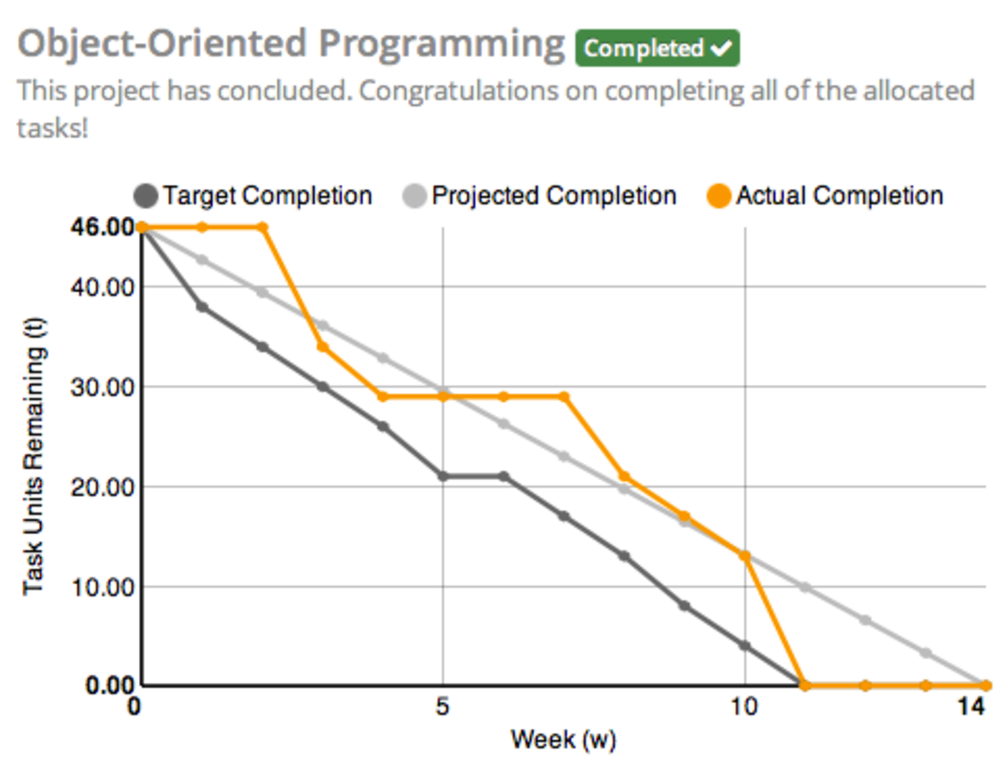
\includegraphics[width=0.8\textwidth]{ExampleChart}
  \caption{An example burn down chart showing progress against weekly tasks}
  \label{fig:example_chart}
\end{figure}

The following list provides an overview of Doubtfire's current features. Each of these features is more fully described in the following section, which describes the features in relation to the associated user roles.
\begin{itemize}[noitemsep,nolistsep]
  \item Individual student progress can be monitored using a Burn Down chart
  \item Collectively, student progress can be viewed in terms of six statuses: \emph{ahead}, \emph{on track}, \emph{behind}, \emph{in danger}, \emph{doomed},\footnote{The ``doomed'' status was a wordplay related to the classic ``Doom'' 3D shooter game, and the notion of incorporating gamification ideas. This status was only visible to staff.} and \emph{haven't started}.
  \item Units, their tasks and students, can be administered allowing tasks and student to be added and removed.
  \item Task status can be updated in response to student work, and staff feedback. 
  \item The tool can be accessed using modern web browser, and provides an adaptable user interface, which caters for both mobile and desktop access.
  \item Role based access, providing appropriate interfaces and actions for teaching staff and students.
\end{itemize}

% subsubsection features (end)

\subsubsection{User Roles} % (fold)
\label{sub:user_roles}

Doubtfire provides functionality for three distinct user roles: Convenor, Tutor and Student. Each of these roles has access to a different set of features, as described in \tref{tab:user_features}. Convenor and Tutor roles support teaching staff, with the students having a separate role. 

% This is what can do with the tool
\begin{table}[htbp]
  \renewcommand{\arraystretch}{1.6}
  \centering
  \caption{Available features for each user group in Doubtfire}
  \label{tab:user_features}
  \begin{tabular}{c|p{0.9\textwidth}}
    Role & \multicolumn{1}{l}{Features} \\ \hline\hline
    \multirow{5}{*}{\begin{sideways}\parbox{35mm}{Convenor}\end{sideways}}
    & \textbf{Unit Administration}: Includes the ability to enrol students and create tasks. \\
    & \textbf{Monitor Student Progress}: View distribution of students by progress indicators. See \fref{fig:dashboard}. \\
    & \textbf{Monitor Task Progress}: View progress distribution for each unit's tasks. See \fref{fig:task_chart_view}. \\
    & \textbf{Examine Student Progress}: View student list showing status for each task. See \fref{fig:tutor_view}. \\
    & \textbf{Update Task Status}: Mark student work as complete. \\ 
    & \\
    \hline\hline
    \multirow{2}{*}{\begin{sideways}\parbox{15mm}{Tutor}\end{sideways}}
    & \textbf{Examine Student Progress}: View student list showing status for each task. See \fref{fig:tutor_view}. \\
    & \textbf{Update Task Status}: Mark student work as complete. \\ 
    & \\
    \hline\hline
    \multirow{3}{*}{\begin{sideways}\parbox{15mm}{Student}\end{sideways}}
    & \textbf{Update Task Status}: Mark student work as complete. See \fref{fig:task_list}. \\ 
    & \textbf{Monitor Progress}: View progress on task completion using a burn down chart showing Target, Actual and Projected completion. \\
    & \\
  \end{tabular}
\end{table}

Unit convenors are responsible for the overall delivery and management of the unit. To support this role, Doubtfire provides convenors with tools to set up tasks and enrol students. A dashboard provides an overview of student progress, and enables quick access to views of student progress by task, and to individual students via scheduled classes. \fref{fig:dashboard} shows an example convenor dashboard overview of students progress within a unit. \fref{fig:task_chart_view} shows an example chart that visualises the distribution of student status for each task. In addition to these tasks, Convenors also have the ability to perform the same actions as Tutors.

\begin{figure}[thbp]
  \centering
  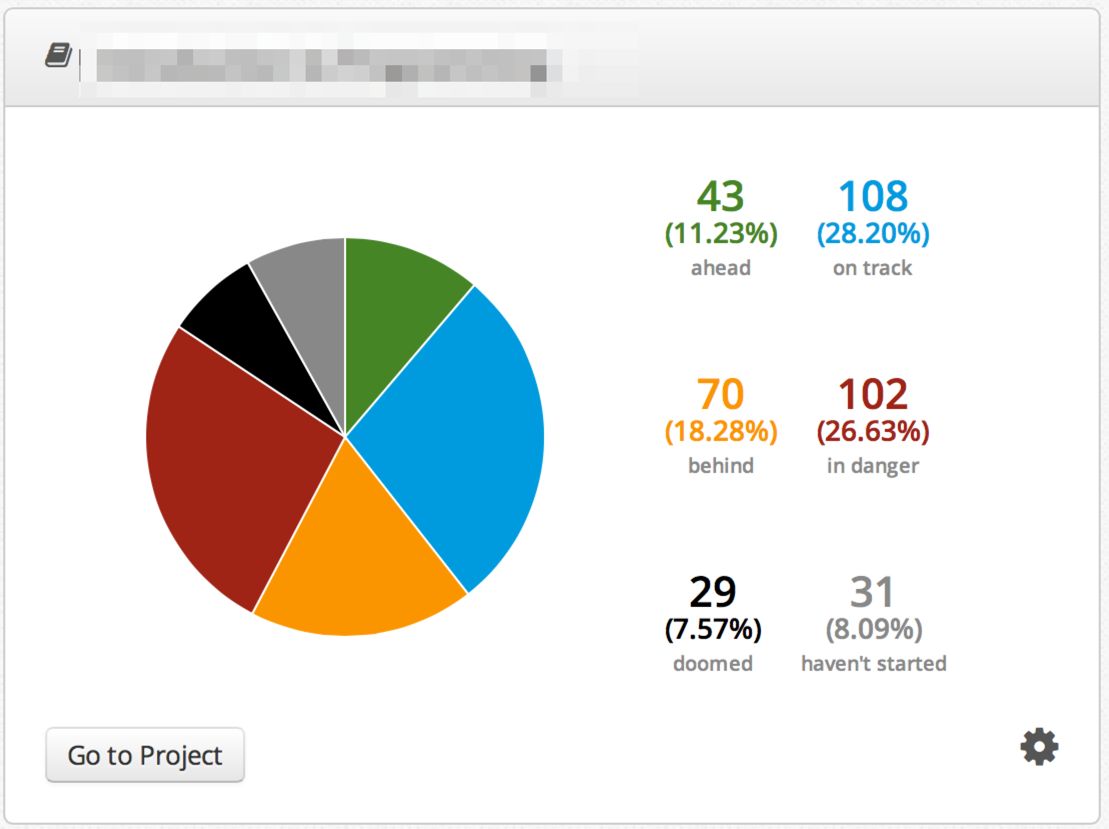
\includegraphics[width=0.8\textwidth]{Dashboard}%
  \caption{Overview of progress by unit from the Convenor Dashboard showing indicators of student progress}%
  \label{fig:dashboard}%
\end{figure}

\begin{figure}[thbp]
  \centering
  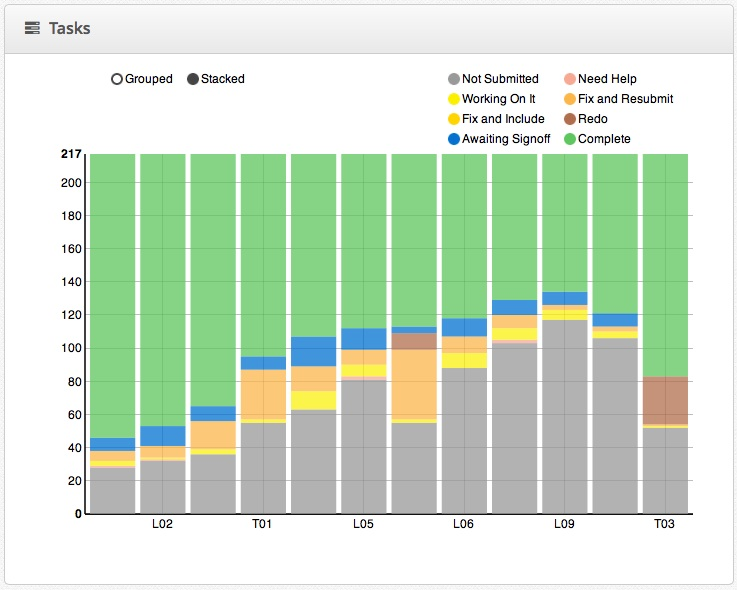
\includegraphics[width=0.8\textwidth]{TaskChart}%
  \caption{Convenor view showing distribution of student status by task, bars can be stacked as shown or grouped by task status.}%
  \label{fig:task_chart_view}%
\end{figure}

Tutors are responsible for conducting the tutorial classes, and providing formative feedback to the students. To support this role, Doubtfire provides tutors with a class-list view showing student progress. From the class list, tutors can drill down to view individual students and their burn down charts. It also provides a convenient means for tutors to update the status of student tasks. 

\fref{fig:tutor_view} shows an example of the class list used by Tutors to view student details and update task status. Each task is represented by a coloured rectangle that indicates the task's current status for that student. Tutors are able to update the status of a student's tasks directly from the class list by selecting the task, and updating it from a list of possible options, also shown in \fref{fig:tutor_view}.

\begin{figure}[thbp]
  \centering
  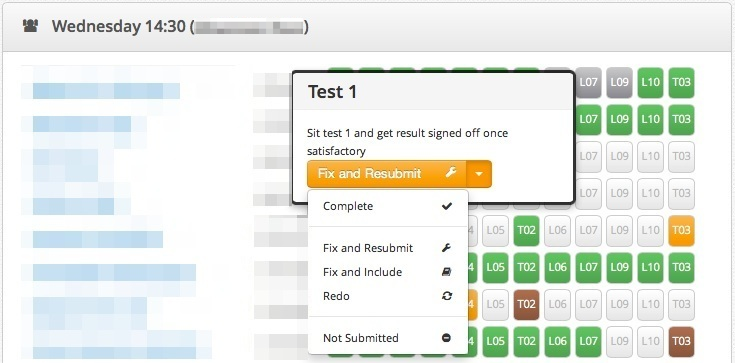
\includegraphics[width=0.8\textwidth]{TutorView}
  \caption{Tutor view of class group, and adjustment of task status. Student names and id numbers have been obscured.}
  \label{fig:tutor_view}
\end{figure}

\fref{fig:home_page} shows an example of the dashboard provided to students, which shows their progress for the units they are enrolled in. For each unit, students can view their burn down chart and each task's status. Students can update the status of a task by selecting it in the task last, and choosing a new status as shown in \fref{fig:task_list}.

\begin{figure}[thbp]
  \centering
  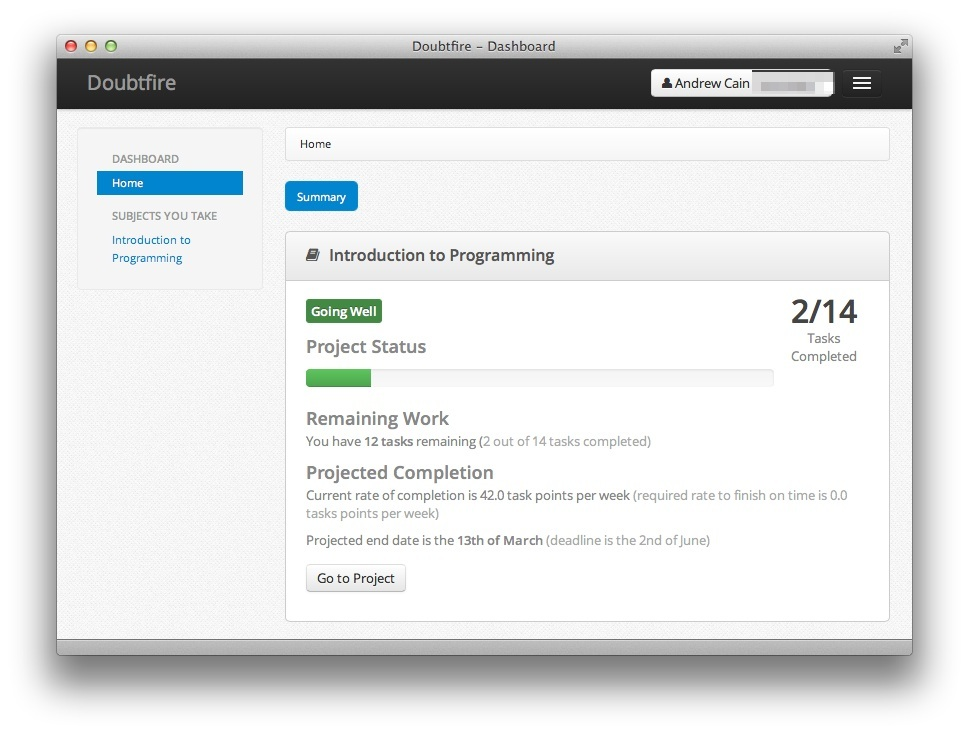
\includegraphics[width=0.9\textwidth]{HomePage}%
  \caption{Student dashboard in Doubtfire showing personal progress for each enrolled unit using the tool}%
  \label{fig:home_page}
\end{figure}

\begin{figure}[thbp]
  \centering
  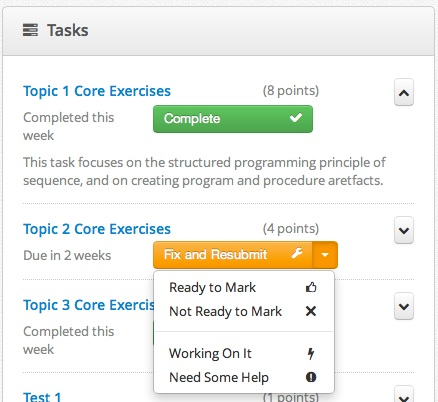
\includegraphics[width=0.5\textwidth]{StudentTasks}
  \caption{The ``Tasks'' list enables students to view and change task status}
  \label{fig:task_list}
\end{figure}

% subsection user_roles (end)

\subsubsection{Task Processes} % (fold)
\label{sub:task_processes}

Tasks in the Doubtfire system have one of a number of states, with different users being responsible for updating task status at various stages during unit delivery. The main states and the transitions between these is shown in \fref{fig:basic_process_chart} as a UML State Chart \cite{OMG:2011}, with additional annotations to indicate user roles reponsible for performing the highlighted transitions. 

\begin{figure}[thbp]
  \centering
  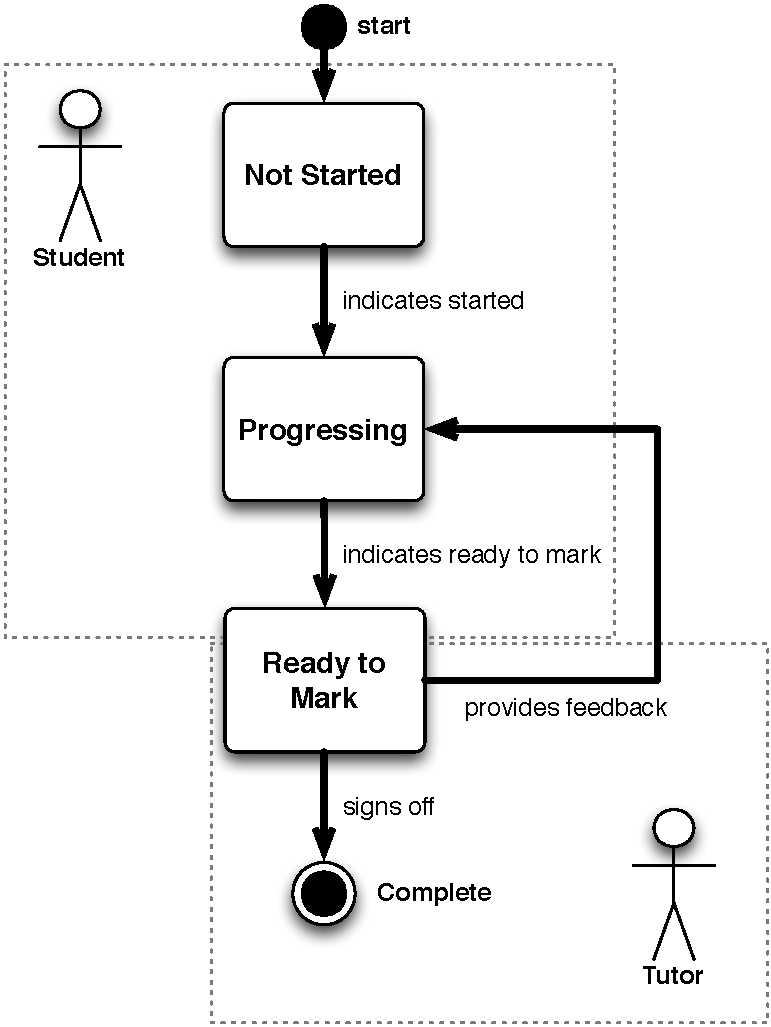
\includegraphics[width=0.7\textwidth]{BasicProcessStateChart}
  \caption{UML state chart showing task states and transitions, and Tutor or Student roles associated with performing these transitions.}
  \label{fig:basic_process_chart}
\end{figure}

Initially all tasks are set to the \emph{Not Started} status. When students begin work on the task they are encouraged to update its status to \emph{Progressing}, and when it is ready for assessment to the \emph{Ready to Mark} status. Once tutors receive the work, they examine the work and provide the student with formative feedback. After having discussed the task with the student, the tutor updates the status by either returning it to a \emph{Progressing} state if the task needs to be fixed, or updating the task as \emph{Complete}.

The \emph{Progressing} status was divided into a number of sub-states for the purpose of providing students with finer-grained feedback. 

Students were able to set the status of a task to \emph{Working on It} or \emph{Needs Help} to indicate their current progress on the task to their tutor and to the unit convenor. \emph{Fix} and \emph{Redo} statuses could be used by students to indicate that tasks needed some aspects adjusted (the \emph{Fix} status) or that it should be redone (the \emph{Redo} status). These status, shown in \fref{fig:detailed_states}, were designed to help provide more accurate details of progress for both staff and students. Students indicated how they were progressing with the tasks, and staff could provide feedback on the outcomes students had achieved.

\begin{figure}[thbp]
  \centering
  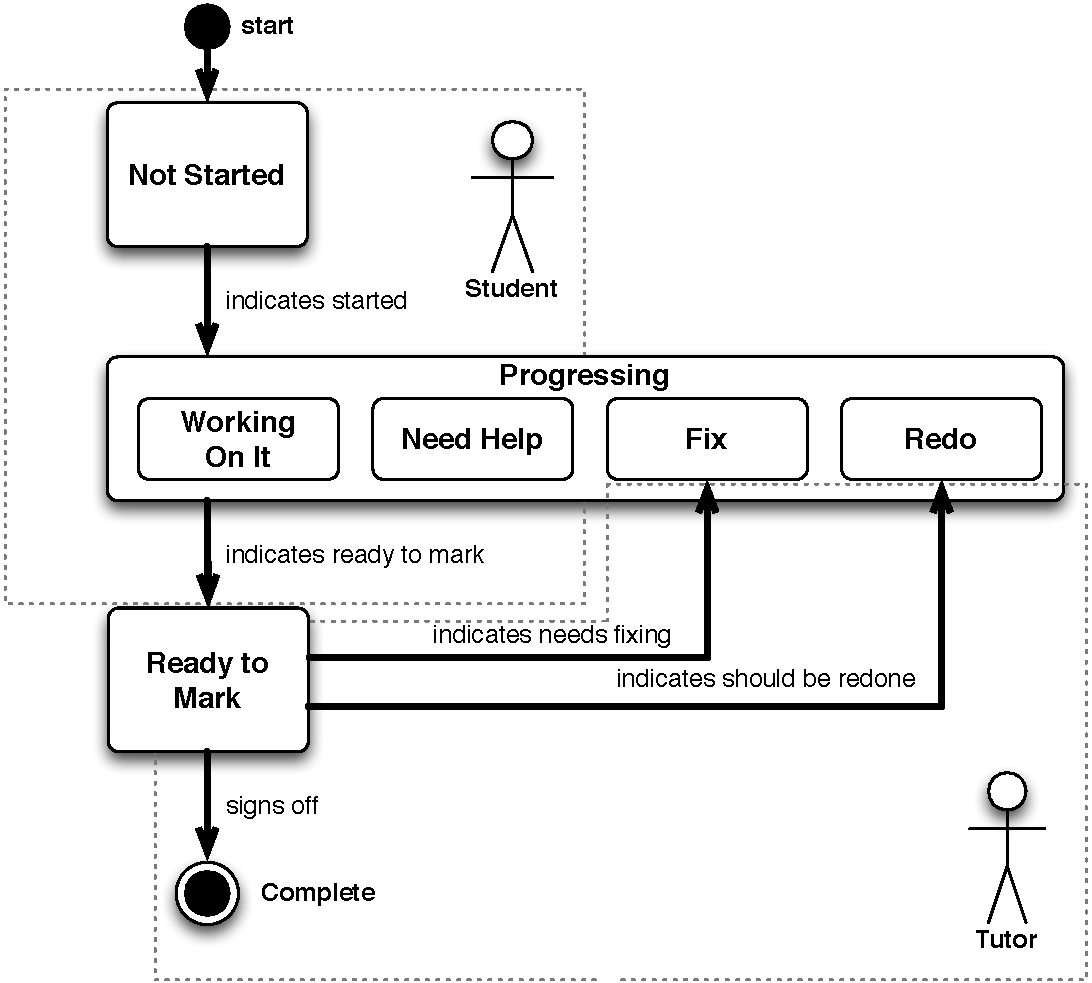
\includegraphics[width=\textwidth]{DetailedStepsInProgress}
  \caption{UML state chart showing the detailed states within the Progressing state}
  \label{fig:detailed_states}
\end{figure}

% subsection doubtfire_solution (end)

\clearpage
\subsubsection{Architecture and Implementation} % (fold)
\label{ssub:architecture_and_implementation}

\fref{fig:doubtfire_arch} provides an overview of the main components of the Doubtfire system. The core of Doubtfire was implemented using Ruby on Rails \cite{Ruby:2013}, with a RESTful API \cite{Richardson:2007}. This encapsulated the core entities -- units, users, and tasks -- and their associated processing. Data is persisted to a MySQL \cite{mysql} database, while an LDAP \cite{Sermersheim:2006} compliant directory server is accessed to provide authentication against the university wide data store.

On the front end, the dynamic nature of the site is achieved though the use of a number of libraries, backed primarily by the jQuery \cite{jquery} JavaScript library. D3.js \cite{d3}, and NVD3 \cite{nvd3}, are used to provide all of the charts, including the burn down charts.  The visual style, and layout, of the website is achieved through use of Twitter Bootstrap \cite{TwitterBootstrap}.

\begin{figure}[htbp]
  \centering
  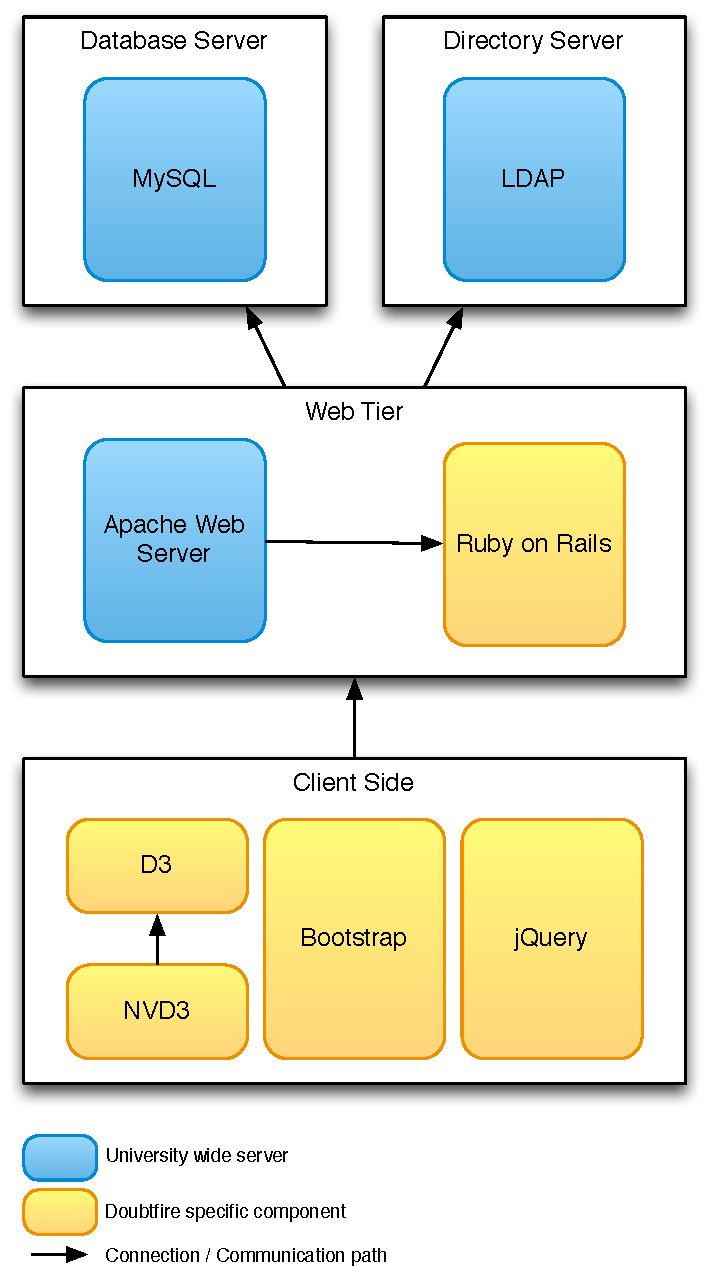
\includegraphics[width=0.5\textwidth]{DoubtfireArch}
  \caption{Overview of main software components in Doubtfire's implementation}
  \label{fig:doubtfire_arch}
\end{figure}

% subsubsection architecture_and_implementation (end)

\subsection{Use and Evaluation of Doubtfire} % (fold)
\label{sub:use_of_doubtfire}

While \cref{cha:evaluation} provides a more in-depth discussion of the use of Doubtfire, this section briefly comments on how it was used in the delivery of the introductory programming and object oriented programming units, and discusses how well its implementation met its requirements. 

Doubtfire has been successfully used in multiple iterations of the programming units described in \cref{cha:example_impl}. In each case, the core tasks from the teaching and learning activities were used as the tasks to be completed, and teaching staff assigned each a t-shirt style weighting to represent its relative size. During unit delivery, students and staff tracked progress against these tasks, with work being signed off by the tutors once complete.

Analysis of student reflections indicated that the effectiveness of the tool, for students, depended on their level of engagement with the unit. Engaged students made active use of Doubtfire, and responded quickly to addressing issues and closing gaps in their knowledge. Students who struggled to complete the weekly tasks generally made poor use of the tool at the start of the teaching period, but engaged actively later in the semester. While some, characteristically disengaged, students avoided use of the system and attempted to establish progress in their own way.

For teaching staff, the Doubtfire tool provided useful information on how students were engaging with the formative process. It was easy to see which students were doing well, to identify those who were falling behind, and those who were not engaging with the unit at all. This information was used to prompt students, encourage those who were doing well and suggest appropriate resources for those who were struggling or falling behind.

In terms of its requirements, Doubtfire was felt to meet its core requirement of providing students with a means of viewing their task progress. The following list outlines the requirements that Doubtfire has met, and those that are currently on the backlog to be implemented in future iterations.

\begin{itemize}[noitemsep,nolistsep]
  \item Requirements met:
  \begin{itemize}[noitemsep,nolistsep]
    \item Staff and students are able to track progress against unit tasks.
    \item Heterogeneous tasks are supported with task weights.
    \item Tasks support a range of states, encouraging students to engage with the system beyond marking work as complete.
    \item Students and staff are able to update task progress based upon their roles.
    \item Student burn down charts show target, projected, and actual completion lines to help indicate likely end dates if current velocity is maintained.
    \item Doubtfire is visually appealing, easy to use, and mobile friendly.
  \end{itemize}

  \item Requirements not implemented:
  \begin{itemize}[noitemsep,nolistsep]
    \item Optional tasks can be entered into the system, but cannot be \emph{acquired} by students.
    \item Gamification ideas were not implement.
    \item Task overviews are provided to staff, but finer-grain detail requires data to be manually exported from the database.
  \end{itemize}
\end{itemize}

In relation to the principles from \cref{cha:guiding_principles}, approach from \cref{cha:approach}, and example units from \cref{cha:example_impl}, Doubtfire provided the following contributions:

\begin{itemize}[nolistsep,noitemsep]
  \item Doubtfire supported the principles by providing:
  \begin{itemize}[noitemsep,nolistsep]
    \item Staff and students with progress data on formative tasks. (\Pref{itm:formative})
    \item Staff will details to help support student learning. (\Pref{itm:support})
    \item Staff with a means of verifying students had completed tasks, without having to revert to marks for motivation. (\Pref{itm:theory_y})
    \item Staff with evidence of student progress that can be used to inform future adjustments to unit delivery. (\Pref{itm:agile} and \Pref{itm:reflect})
    \item Students with progress details they can reflect upon in their Learning Summary Reports. (\Pref{itm:reflect})
  \end{itemize}
  \item Doubtfire supported the approach, and example units by:
  \begin{itemize}[noitemsep,nolistsep]
    \item Encouraging students to engage in the formative feedback process.
    \item Providing evidence that students had completed core tasks.
    \item Enabling staff to identify students who needed additional help and encouragement.
  \end{itemize}
\end{itemize}

\subsection{Summary} % (fold)
\label{sub:doubtfire_summary}

The strong use of formative feedback in the model provides a challenge as students cannot be motivated to work by the fear of losing marks during the teaching period. This can lead to students allocating insufficient time to complete learning activities, resulting in them falling behind in the unit.

Doubtfire was designed to address these concerns through the use of agile development burn down charts that visually represented the amount of work students had remaining in the unit. By using this tool staff and students were able to monitor progress throughout the teaching period.

% subsection summary (end)

% section doubtfire_using_burndown_charts_to_support_formative_feedback (end)
\clearpage
\section{A Game Library to Support Procedures First} % (fold)
\label{sec:swingame}

\cref{cha:example_impl} described two programming units implemented using the approach described in \cref{cha:approach}, and principles stated in \cref{cha:guiding_principles}. Following \pref{itm:paradigm}, these units were each centred around concepts associated with a single programming paradigm. As described in \sref{sec:paradigm_choice}, an objects-later approach was adopted for the introductory programming unit, which focused on introducing students to the procedural programming paradigm, with the subsequent object oriented programming unit introducing the object oriented paradigm.

\pref{itm:concepts} indicates the desire to structure the programming curriculum around programming concepts in such a way that each topic builds upon prior knowledge. This lead to the procedures first approach for the introductory programming unit described in \sref{ssub:procedures_first_topic_sequence}. 

With the procedures first approach to teaching introductory programming, students are introduced to calling and creating procedures before being introduced to other programming concepts. This approach promotes a focus on \textbf{sequence} in these early tasks, with students creating procedures to group together a sequence of procedure calls that perform a certain task. 

The challenge with this approach, as identified by \citet{Pattis:1993}, is finding meaningful tasks for students to perform. Standard programming language features do not provide sufficient functionality for student to perform meaningful, and engaging, actions without having to use a wider range of programming constructs.

This section describes SwinGame \cite{swingame} a game development library designed to facilitate a procedure first introduction to programming, and to help students create more interesting programs. \sref{sub:swingame_requirements} outlines the requirements for the SwinGame library, which is then described at a high level in \sref{sub:swingame_solution}. \sref{sub:use_of_swingame} describes how SwinGame was used to support the teaching of introductory programming, and relates this to the principles, approach, and units from chapters \ref{cha:guiding_principles} to \ref{cha:example_impl}. The discussion of SwinGame concluded with a short summar in \sref{sub:swingame_summary}

\clearpage
\subsection{Requirements} % (fold)
\label{sub:swingame_requirements}

SwinGame was created to help teaching the introductory programming unit described in \cref{cha:example_impl}. The main goal for SwinGame was to provide students with resources to enables them to create more engaging programs, while also providing support for a procedures-first approach to the programming curriculum.

The requirements for SwinGame were to:
\begin{itemize}[noitemsep, nolistsep]
  \item Provide functions, procedures, and custom types to enable the creation of small two dimensional games. Including:
  \begin{itemize}[noitemsep,nolistsep]
    \item Resource management for images, sounds, animations, and maps.
    \item Drawing operations to draw primitive shapes, images, and text.
    \item Sprite management, enabling the creation of movable, animated, game entities.
    \item Ability to play sound effects and music.
    \item Collision detection operations including collisions of geometric shapes, and pixel level image collisions (image-image, and image-shape collisions).
    \item Support for two-dimensional game physics.
    \item Input handling routines to support keyboard, mouse, touch, accelerometer, and gyroscope input.
    \item Time tracking, and management.
    \item Camera support, enabling game space coordinates to be mapped to screen coordinates for drawing.
    \item Network support to enable peer-to-peer interactions, as well as enabling http requests to get/post high score details to web servers, for example.
  \end{itemize}
  \item Give the programmer full control over the game's actions, requiring explicit requests to perform any task.
  \item Enable developers to develop their programs on a number of platforms: Linux, MacOS, and Windows.
  \item Enable programs to be run on a number of devices: Desktop computers, tablets, and smart phones. 
  \item Be implemented in such a way that it can be developed and extended by students.
  \item Provide access to the functionality across a range of programming languages, ensuring that each language provides appropriate programming abstractions to ensure that the library can be used appropriately. (\Pref{itm:authentic})
\end{itemize} 

% subsection requirements (end)
\clearpage
\subsection{SwinGame Solution} % (fold)
\label{sub:swingame_solution}

% SwinGame is a game development library designed to support the teaching of introductory programming. Commercial game development tools focus on performance and productivity, removing control from the programmer in order to improve both and to avoid boilerplate code. In contrast, the goals of SwinGame focus on enabling students to explore programming concepts, while at the same time creating programs that are fun and engaging. 

\fref{fig:swingame_overview} provides an overview of the components involved in the use of development of the SwinGame library. The library itself, provides students with an interface that, to procedural programming languages, exposes a range of functions and procedures that can be called to perform required actions. The logic of SwinGame itself is divided into \emph{Core Logic}, and \emph{Back-end Logic}. The components in the Core Logic implement the higher level game engine mechanics, while the components in the Back-end Logic provide a consistent interface to lower level third party components.

\begin{figure}[htbp]
  \centering
  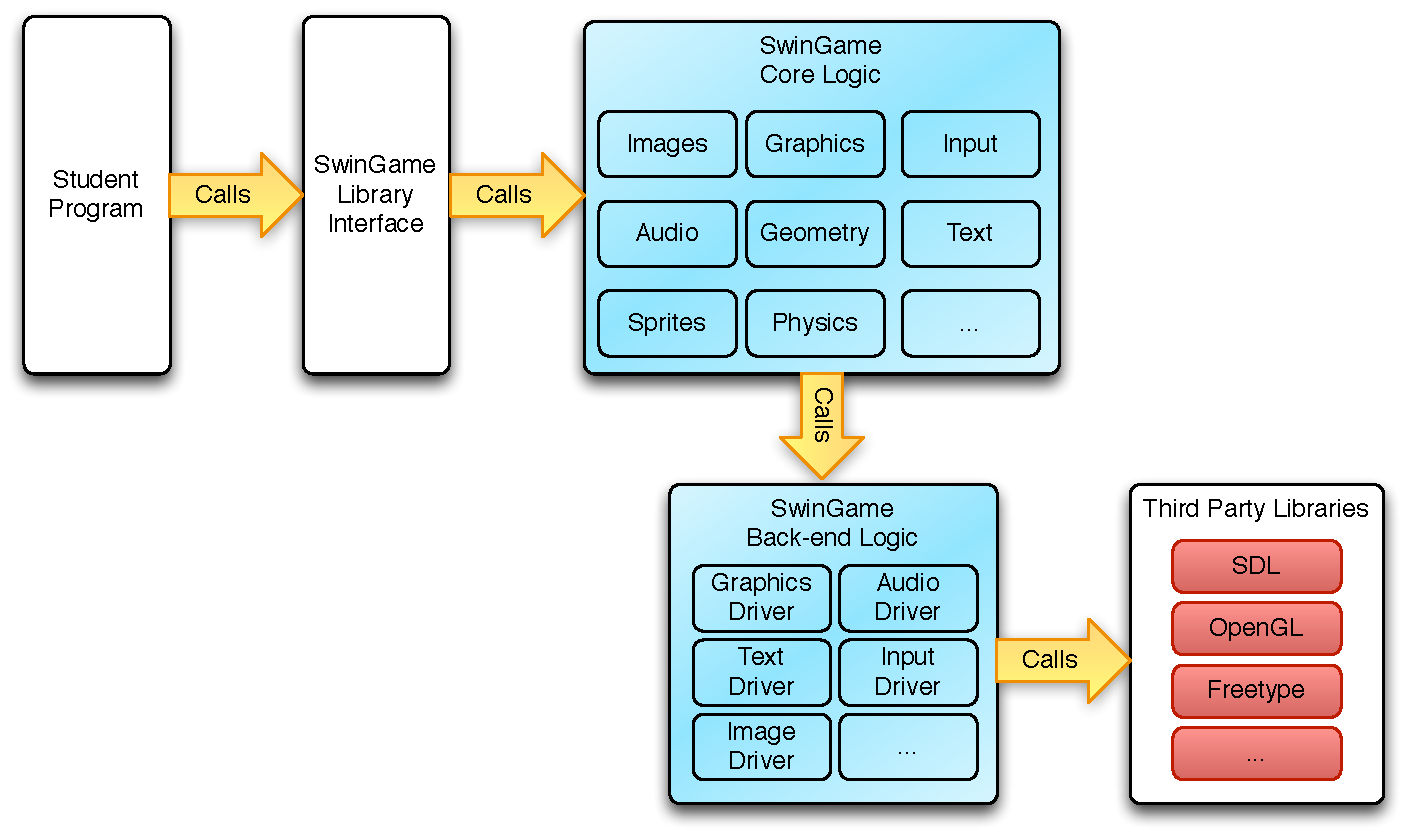
\includegraphics[width=\textwidth]{SwinGameOverview}
  \caption{Overview of the components in the SwinGame library, their connections and organisation.}
  \label{fig:swingame_overview}
\end{figure}

The division of SwinGame, into Core Logic and Back-end Logic, decouples the core game engine logic from the lower level libraries used. This enables the library to update Back-end components with minimal impact on the core logic. Currently SwinGame supports a number of different back-end components used to support different platforms and underlying third party libraries.

SwinGame provides users with a number of components and features. The main components are briefly outlined in the following list.
\begin{itemize}[noitemsep,nolistsep]
  \item \textbf{Animations}: provides the ability to load and play cell based animations.
  \item \textbf{Audio}: supports loading and playing of sound effects and music.
  \item \textbf{Camera}: enables a virtual camera to be moved around the game world -- adjusting what is shown by mapping game to screen coordinates.
  \item \textbf{Geometry}: provides mathematical operations to manipulate geometric shapes.
  \item \textbf{Graphics}: enabling a window to be opened and providing functions to draw geometric shapes.
  \item \textbf{Images}: supports loading and drawing bitmap images.
  \item \textbf{Input}: supports keyboard, touch, and accelerometer input.
  \item \textbf{Networking}: provides the ability to create and use network connections.
  \item \textbf{Physics}: provides functions to perform collisions between entities.
  \item \textbf{Resources}: supports the management of image and sound resources, mapping names to resources.
  \item \textbf{Sprites}: enables the creation of image based sprites.
  \item \textbf{Text}: supports font loading, and text rendering.
  \item \textbf{Timers}: provides access to components to track and manage time based actions.
  \item \textbf{User Interface}: enables creation of user interfaces including labels, text boxes, lists, buttons, and other components.
  \item \textbf{Utilities}: provides other miscellaneous operations useful for game development.
\end{itemize}

% subsection swingame_solution (end)

\subsection{Use and Evaluation of SwinGame} % (fold)
\label{sub:use_of_swingame}

\subsubsection{Supporting Early Exercises and Lecture Demonstrations} % (fold)
\label{sub:supporting_early_exercises}

SwinGame was used to support the early exercises in the teaching and learning activities for the introductory programming unit described in \cref{cha:example_impl}. For example, procedures were introduced in Week 1 where students developed a small program that drew a house, the resulting code from this exercise is shown in \lref{lst:house_drawing}. This task aims to focus students attention on concepts related to procedure declarations, procedure calls and instruction sequence. Sequence was explored by adjusting the order of the instructions in the program, and examining the results on the images drawn. Core exercises in Week 1 then built on this, having students complete a program that used images and sound effects to deliver a joke, the starting code for which is shown in \lref{lst:joke}. Screen-shots of the resulting programs are shown in \fref{fig:week1_progs}.

\passection{lst:house_drawing}{The Pascal code for the House Drawing laboratory exercise from the introductory programming unit. In this program students explored concepts related to procedures and sequence.}{\pascode{Figures/Supporting/HouseDrawing.pas}}

\passection{lst:joke}{The core exercise in Week 1 of the introductory programming unit had students complete a program that told a joke. This included code to draw images, play sound effects and draw text.}{\pascode{Figures/Supporting/KnockKnock.pas}}

\begin{figure}[thb]
  \centering
  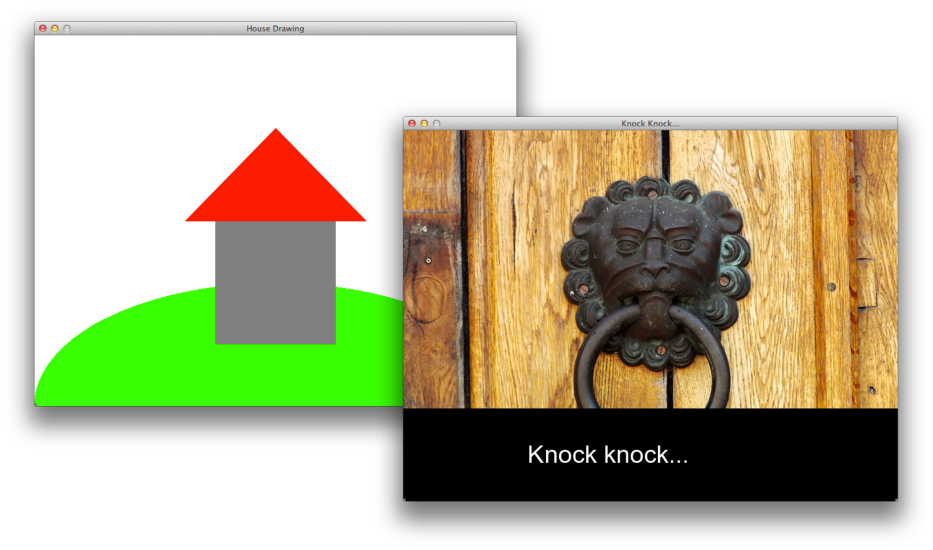
\includegraphics[width=\textwidth]{Week1Progs}
  \caption{The programs created in Week 1 of the introductory programming unit}
  \label{fig:week1_progs}
\end{figure}

With the students in full control of their programs, any form of user interaction required students to implement their own event handling loop. This provided a convenient motivation for control flow mechanisms in Week 3 of introductory programming. By this point, students could create parametrised procedures to draw shapes, but program duration was always set by the length of the delay coded into the sequence. By introducing \textbf{repetition} it became possible to keep a window open \emph{until} the user asked for it to close. With \textbf{selection} user actions could then be responded to, updating values in variables that changed how things were drawn on the screen.

The visual nature of the games developed with SwinGame help create a more engaging atmosphere in lectures. By creating visual programs, the lecture demonstration code can be designed and implemented \emph{with} the students. For example, in Week 3 of the introductory programming unit the lecture demonstration created a small program where the user could move a light around the screen and turn it on and off. The code in \lref{lst:lights} shows a part of the code developed in this lecture. The program was created iteratively, involving the students at each stage, as outlined in the following list.

\begin{enumerate}[noitemsep, nolistsep]
  \item Initially the program was developed using concepts from previous week, with the code implementing the \texttt{DrawLight} procedure. At this stage a call to \texttt{Delay} was used to keep the program open for a short period. In this way the example helps build upon student's prior knowledge. (\Pref{itm:concepts})
  \item The first problem was highlighted by explaining how the program worked, while it was running. Half way through the explanation the program ended, leading to the question ``How can we keep the program open until we want it to close?''. Via various prompts the event loop was described, and coded as the repeat loop in main. Counting out a period longer than the previous delay highlighted that the new code had solved the old problem, and the class discussed what was actually happening behind the scenes to enable this. Closing the window demonstrated the ending of the repeat loop.
  \item The next problem was to make the program more interactive: ``Wouldn't it be good to be able to turn the light on and off?''. This lead to a discussion of what needed to \emph{vary} in the program, and the addition of the \texttt{lightIsOn} variable in \texttt{Main}. This was set to false when the program started, and its state was flipped (on to off, and visa versa) in the repeat loop.
  \item Running the program had an \emph{interesting} effect, as the light flickered between its two states. Questions started with ``Do we always want to change the state of the light?'', and eventually lead to ``So, you only want to change the state of the light \textbf{if} the user has typed the space bar?'' and follow on to ``How can we achieve this in our code?''. After reviewing selection, and the syntax for the if statement, the assignment statement that changed the lights state was put within an if statement. The program was executed and the results discussed.
\end{enumerate}

Other features were added in a similar style, each focusing on the application of the concepts to solve a problem or to introduce a new feature.  The exercise demonstrates the application of constructive learning theories (\Pref{itm:construct}) , in that it aims to help guild students in the construction of their knowledge. The example starts at a point they should be familiar with, and identifies ways in which the new knowledge, control flow in this case, can enhance the functionality of the program they are creating (\Pref{itm:concepts}). In this way, the examples demonstrate appropriate applications of the new concepts, helping students work toward the goal of thinking and acting as experts.

\passection{lst:lights}{The final code from the lecture example developed with students in the Week 3 lecture of the introductory programming unit. The program shows a light bulb image that can be turned on and off with the mouse and space bar, and moved around the screen using arrow keys.}{\pascode{Figures/Supporting/Lights.pas}}

Each week's lecture demonstrations followed a similar sequence. SwinGame enabled the focus on programming concepts (\Pref{itm:concepts}) due to its requirement for explicit control, while its support for multimedia resources helped make the programs more ``fun.'' Later week's lecture demonstrations continued to expand on concepts learnt, and culminated in the development of a small game. The functionality and theme of these games were proposed by students, helping them take ownership of the learning activities (\Pref{itm:theory_y}). Students supplied images and sound effects, suggested features, discussed implementation strategies and were engaged in the iterative implementation of these games. \fref{fig:games} shows screen-shots of two games developed in the lectures, the code of which was then shared with the students.

\begin{figure}[thbp]
  \centering
  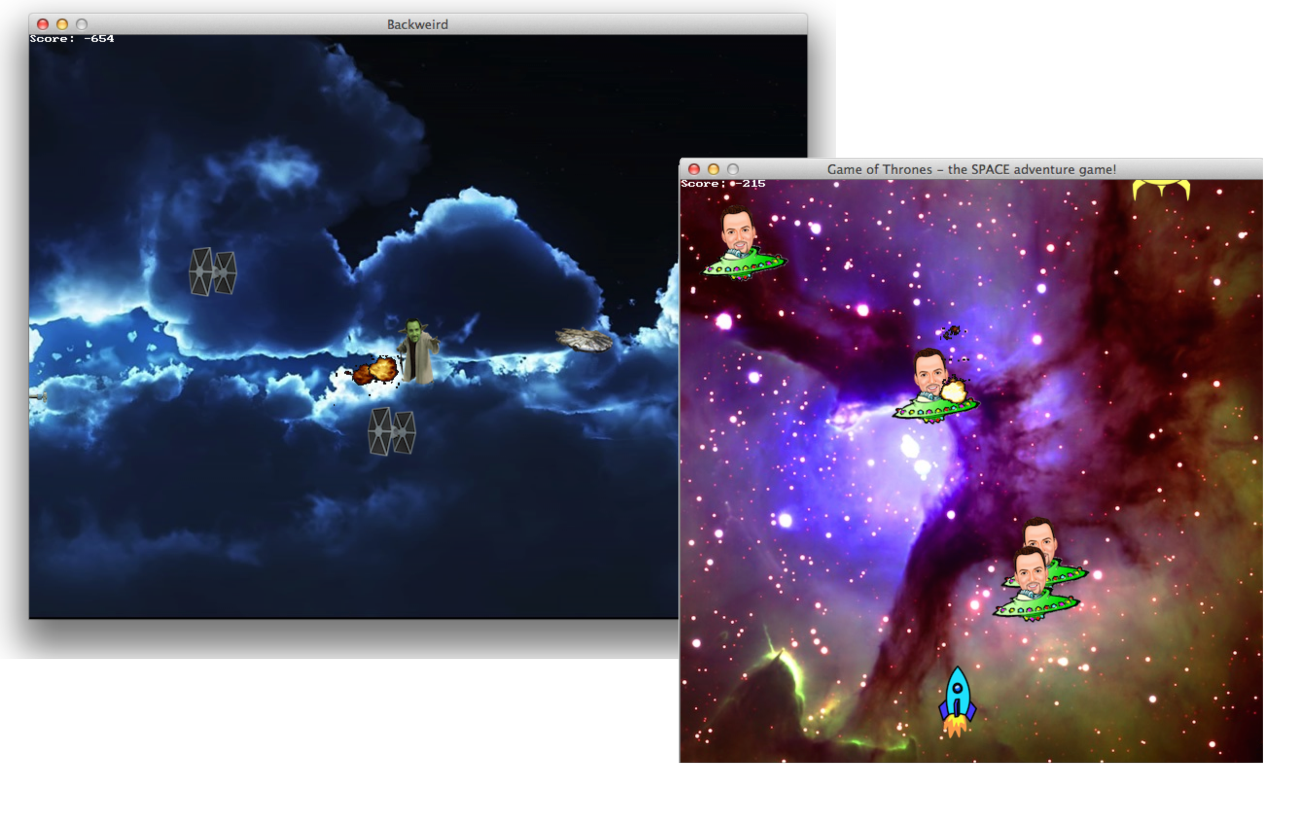
\includegraphics[width=\textwidth]{Games}
  \caption{Games developed with students across a number of weeks in introductory programming}
  \label{fig:games}
\end{figure}

% subsection supporting_early_exercises (end)

\subsubsection{Supporting Custom Projects} % (fold)
\label{sub:supporting_custom_projects}

As well as supporting the delivery of lecture material, SwinGame provided students with a wide range of capabilities they could use in the creation of their \emph{custom projects}. The assessment criteria developed for the introductory programming unit, described in \sref{sub:intro_constructing_assessment_criteria}, required students to demonstrate they could apply the concepts from the unit to develop a program of their own design. While there was no requirement for students to use the library, most chose to create a game using SwinGame.

To help support students with their use of SwinGame was documented on a website \cite{swingame}, as shown in \fref{fig:website}. The website was created to list the SwinGame functions and procedures, and additional documentation was added for some of the more common tasks, with the aim of supporting students as they started to develop their own programs (\Pref{itm:support}). The site also provided a means of distributing the SwinGame library to a wider audience.  

\begin{figure}[thbp]
  \centering
  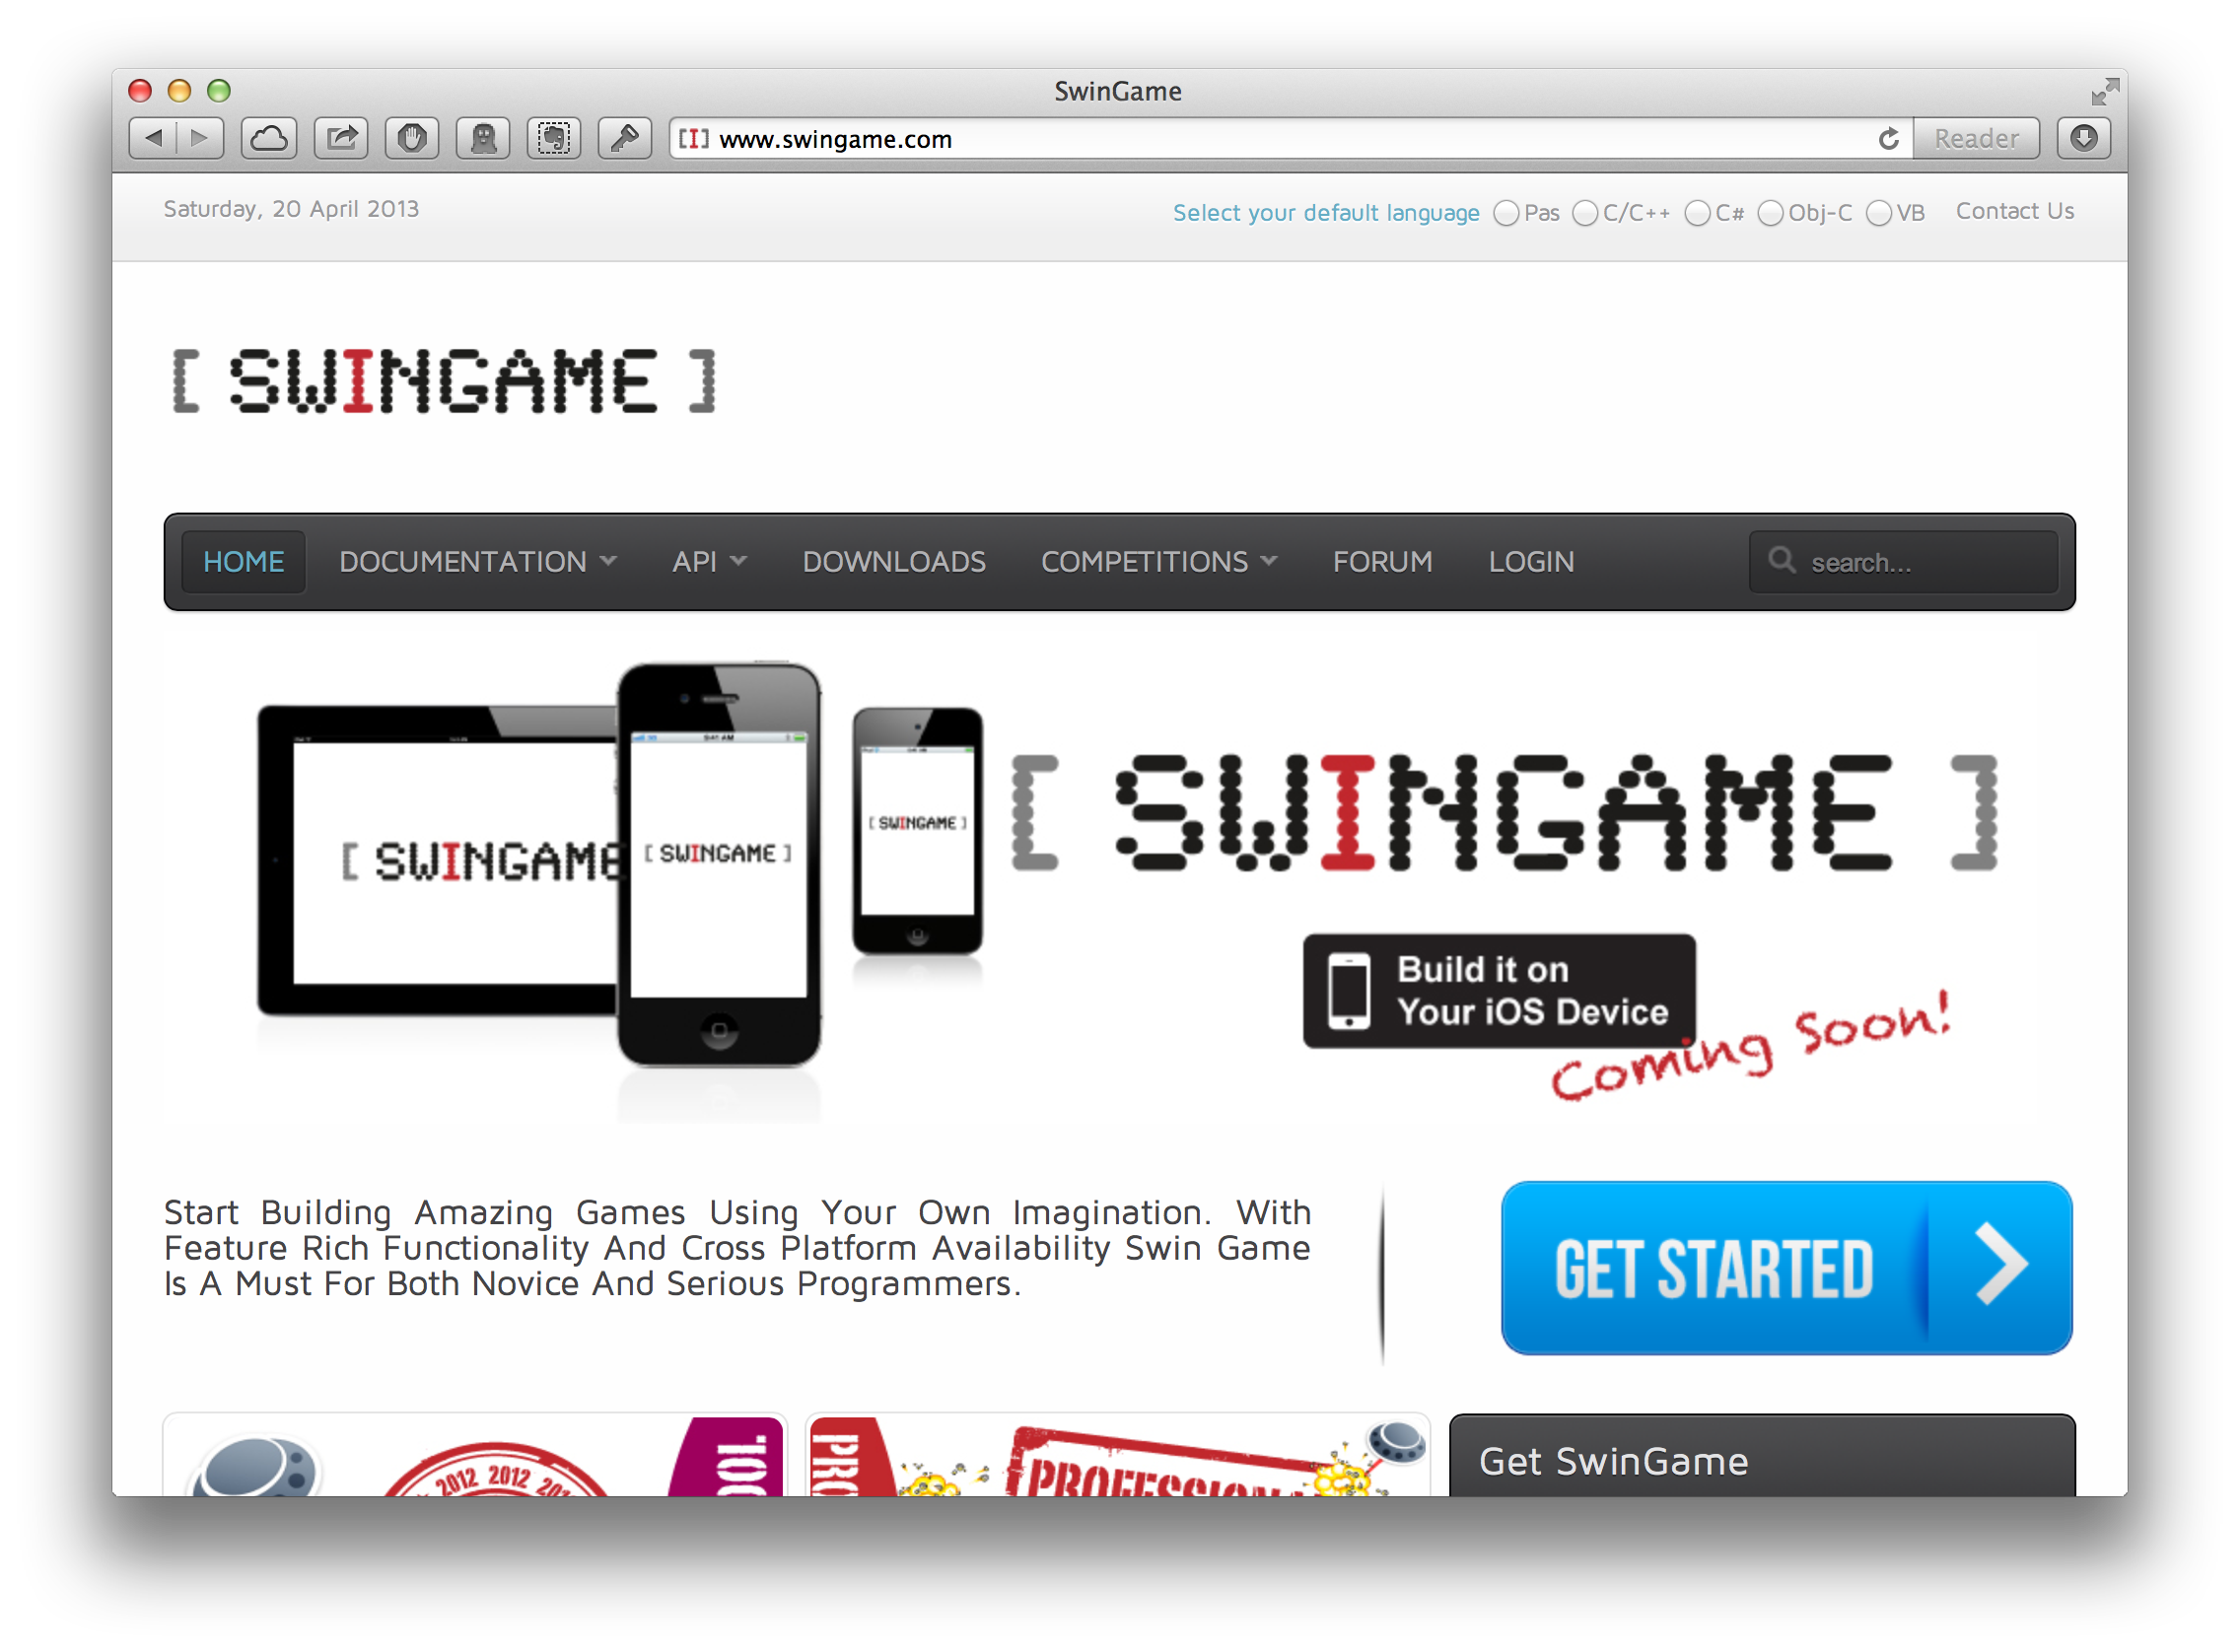
\includegraphics[width=0.9\textwidth]{SwinGame}
  \caption{The SwinGame website provides a means of distributing SwinGame and its documentation}
  \label{fig:website}
\end{figure}

% subsection supporting_custom_projects (end)

\subsubsection{Developing SwinGame and its Documentation} % (fold)
\label{sub:developing_swingame_and_its_documentation}

SwinGame was developed through the collaboration of both staff and students over a number of years. At the end of each year, students were invited to work on enhancing SwinGame's implementation and documentation. This provided an opportunity for staff to work closely with students, and for students to further develop their software development skills outside of the standard teaching periods.

Promoting opportunities to work on SwinGame also provided an opportunity to indicate the depth of knowledge students had developed in the past. This helped communicate the high expectations of staff (\Pref{itm:expectations}) and provided encouragement for students to do their best.

% subsection developing_swingame_and_its_documentation (end)

\subsubsection{Supporting Multiple Languages} % (fold)
\label{sub:supporting_multiple_languages}

With the introductory programming unit using two programming languages, and object oriented programming using four, SwinGame was required to be accessible from a range of programming languages. This included both procedural and object oriented programming languages, which each needed to be supported with appropriate abstractions (\Pref{itm:authentic}). To achieve this goal a number of tools were created to simplify the process of creating programming language specific versions of SwinGame.

SwinGame's core logic can be accessed via language specific wrappers as shown in \fref{fig:swingame_arch}. Each wrapper mirrors the SwinGame functionality, and acts as an adapter that performs any required transformation of data between the program's runtime environment and the native SwinGame library, which is accessed via the SwinGame Library Interface. This interface consolidates all of the SwinGame functionality and exposes it as a native library, it also acts as an adapter that converts SwinGame types to, and from, appropriate native representations that can be exchanged across the native interface. 

\begin{figure}[thbp]
  \centering
  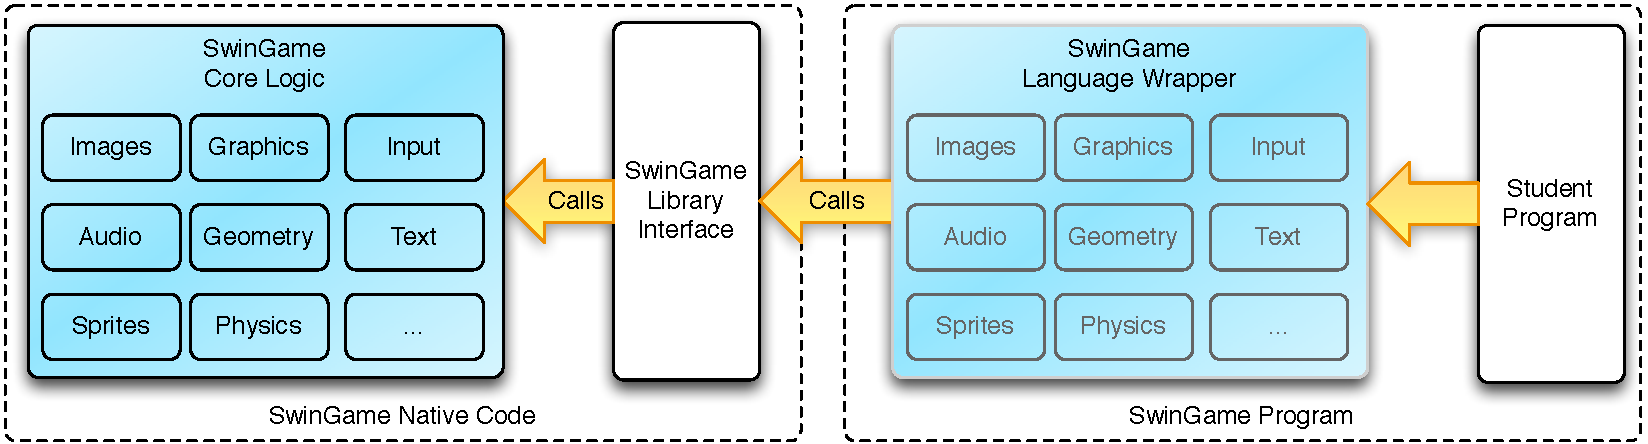
\includegraphics[width=\textwidth]{SwinGameArch}
  \caption{SwinGame core logic is implemented in a number of modules that are accessible via language specific wrappers }
  \label{fig:swingame_arch}
\end{figure}

To ease the creation of the language specific wrappers a translator was created that reads the source code of the SwinGame core logic and outputs the SwinGame Library Interface, a number of matching language specific wrappers, and the programmer documentation for the SwinGame website, as shown in \fref{fig:swingame_trans}. This ensures consistency between the wrapper, SwinGame Library Interface and the documentation, while allowing the development of SwinGame to focus on enhancing the core logic.

\begin{figure}[thbp]
  \centering
  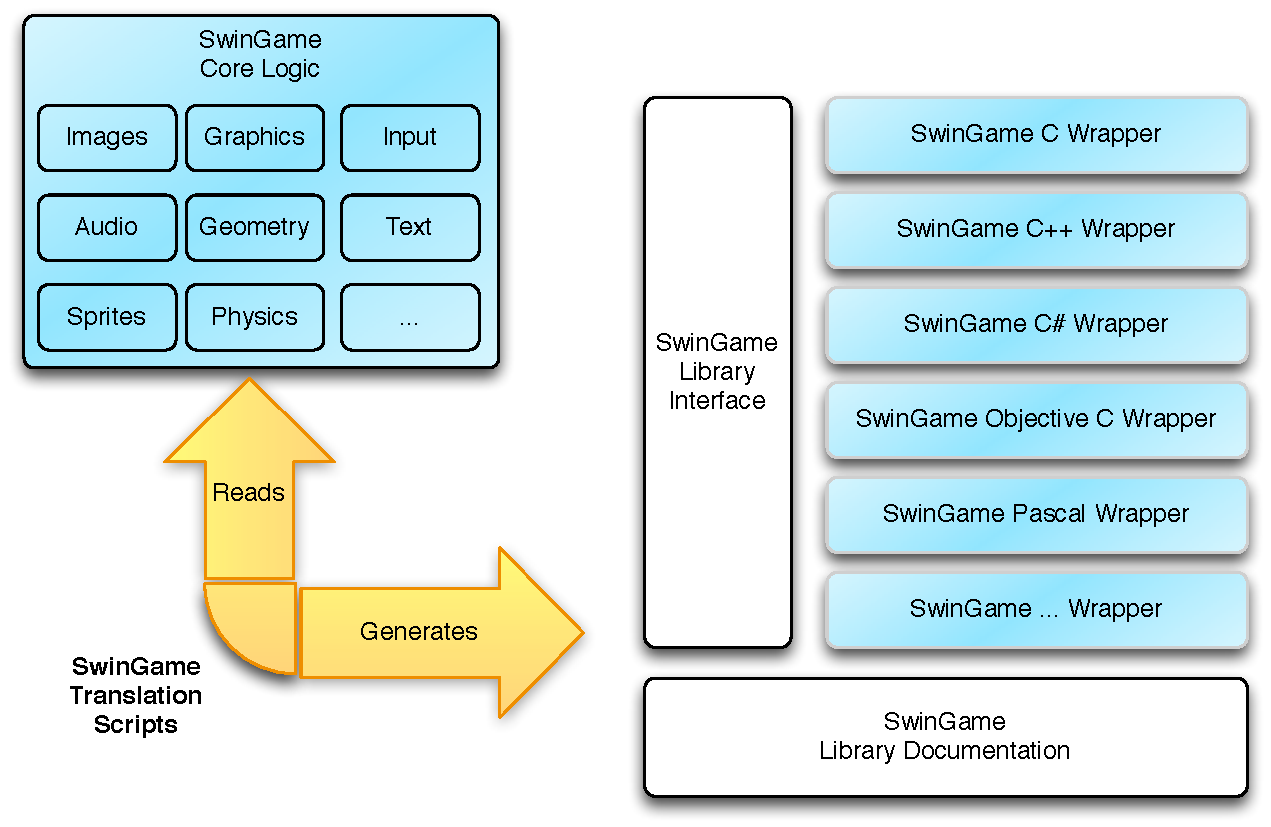
\includegraphics[width=\textwidth]{SwinGameTranslator}
  \caption{SwinGame's language specific wrappers, library interface and programmer documentation are all generated from its source code. The translator reads the source code, and outputs the SwinGame library, and language specific wrappers for a range of programming languages.}
  \label{fig:swingame_trans}
\end{figure}

SwinGame's language translation scripts requires additional information to enable the construction of the various artefacts. It was decided to store these additional details using attributes in comments in the code of the core logic. These special comments started with \texttt{///} and contained documentation as well as other information needed to assist with the translation. These attributes were marked using the \texttt{@} symbol followed by a attribute identifier and a number of values. Two example functions from the SwinGame core logic are shown in \fref{lst:audio}, and \tref{tbl:attributes} provides details of the attributes shown.

\passection{lst:audio}{Example of markup language used to annotate SwinGame core logic to enable generation of language specific wrappers}{\pascode{Figures/Supporting/Audio.pas}}

\begin{table}[htbp]
    \footnotesize
    \centering
    \caption{The main language translation attributes, their format and purpose.}
    \label{tbl:attributes}
    \begin{tabular}{l|l|p{8cm}}
    Attribute & Format & Purpose \\
    \hline
    \texttt{@param} & \texttt{@param name docs} & Provides additional documentation for a parameter. \\
    \texttt{@lib} & \texttt{@lib} & Indicates the function/procedure should appear in the SwinGame Library Interface. \\
    ~ & \texttt{@lib call} & Indicates that the wrapper should call another function/procedure from the SwinGame Library Interface. \\
    \texttt{@uname} & \texttt{@uname name} & Function and procedure names in the SwinGame Library Interface, and some wrappers, need to be unique. This attribute provided a unique name for this function or procedure. \\
    \texttt{@sn} & \texttt{@sn format} & Provides a format string for the creation of the Objective C signature for this function/procedure. This allows parameters to be mixed with the name of the method. \\
    \texttt{@class} & \texttt{@class name} & The name of the class to add the method to. \\
    \texttt{@method} & \texttt{@method} & The name of the method to add to the class. \\
    \texttt{@overload} & \texttt{@overload name uname} & Overloads the method name, uname is used in langauges that do not support overloading. \\
    \texttt{@csn} & \texttt{@csn format} & Similar to @sn, providing the format for the Objective C signature for the method added to the class. \\
    \end{tabular}
\end{table}

The \texttt{@lib} parameter determines if the function or procedure is added to the SwinGame Library Interface. When the function or procedure is not to be added, an alternative call is provided. The generated wrapper code is then adjusted to call the appropriate function. The code in \fref{lst:audio} indicates that \texttt{LoadSoundEffect} should be included directly in the interface, whereas this version of the \texttt{PlaySoundEffect} procedure calls \texttt{PlaySoundEffectA} and passes in default values for some parameters.

All SwinGame resources are accessible via pointers, enabling the language translation scripts to create object oriented abstractions when this is appropriate for the wrapper's programming language. \fref{fig:swingame_wrapper_output} illustrates the main components created by the translator. 

Each function and procedure in the core logic is capable of creating two methods in the object oriented language wrappers. The first method is created as a static\footnote{Static in this context is meant to indicate that the method is associated with the class, rather than instances of the class.} member of a class that mirrors the module from the core logic. The second method can then be associated with a matching resource class, as an instance member. The specific class is indicated by the \texttt{@class} attribute. These classes contain a field to track the resource's pointer, and so the method will have one fewer parameters. When these methods are called, they calls the matching method static method and pass in the value from the pointer field along with any other parameter values passed to the method.

\begin{figure}[thbp]
  \centering
  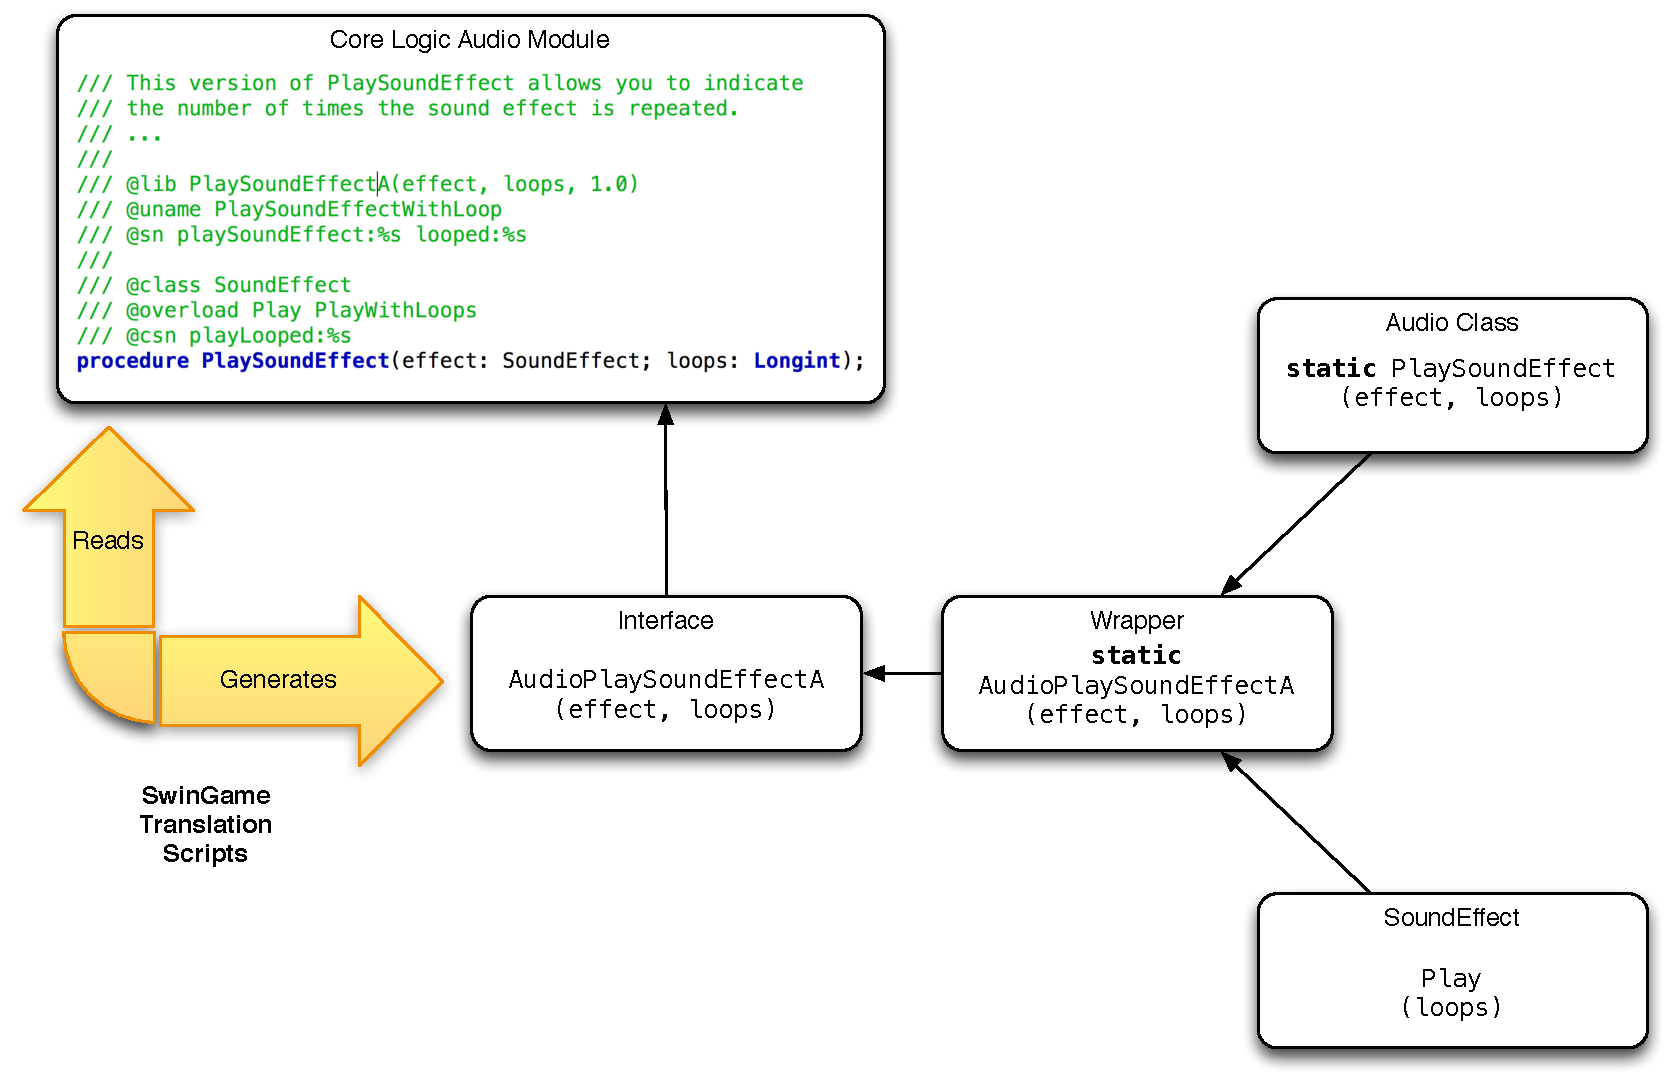
\includegraphics[width=\textwidth]{SwinGameWrapperOutput}
  \caption{Attributes in the core logic code define the generation of a module level wrapper, and the creation of classes for object oriented access to SwinGame resources.}
  \label{fig:swingame_wrapper_output}
\end{figure}

The Objective C syntax required special attention, as method signatures do not separated name from parameters. For example, the procedure PlaySoundEffect shown in \fref{lst:audio} could be called using \texttt{[Audio playSoundEffect:effect looped:3]}. The signature to match this required the parameters to be embedded within the method's name. This was achieved by adding \texttt{@sn} and \texttt{@csn} attributes that allow the developer to specify a format string into which the parameter signatures are injected.

By supporting both procedural and object oriented programming languages, SwinGame was able to be used in both the introductory programming and object oriented programming units. In introductory programming students worked with SwinGame from Week 1, and explored its use from both the Pascal and C programming languages. In the object oriented programming unit, SwinGame provided a familiar framework for students to work with at the start of the teaching period. As the teaching period progressed, students were transitioned away from using SwinGame to encourage them to explore other commercially available libraries by the end of the unit.

% subsection supporting_multiple_languages (end)
\subsubsection{Supporting What We Teach} % (fold)
\label{sub:supporting_what_we_teach}

SwinGame performed a central role in supporting \emph{what} was taught in the two example programming units described in \cref{cha:example_impl}. It also provided backing for other resources developed to support the teaching of these units, as illustrated in \fref{fig:what_we_teach}. SwinGame helped enable interactive lectures, and provided the tools necessary to create engaging examples in the Programming Arcana text, outlined in \sref{sec:arcana}, and the video podcasts, described in \sref{sec:vodcasts}. 

It also provided a consistent library for students to use as they moved between programming languages, and programming units (\Pref{itm:support} and \Pref{itm:concepts}). While the SwinGame interface differed slightly, adapting to language conventions and abstractions, the interface was still a familiar quantity as students moved between languages and paradigms. This meant that students could more rapidly create programs in the new language, as the SwinGame library remained relatively consistent between the different environments.

\begin{figure}[thb]
  \centering
  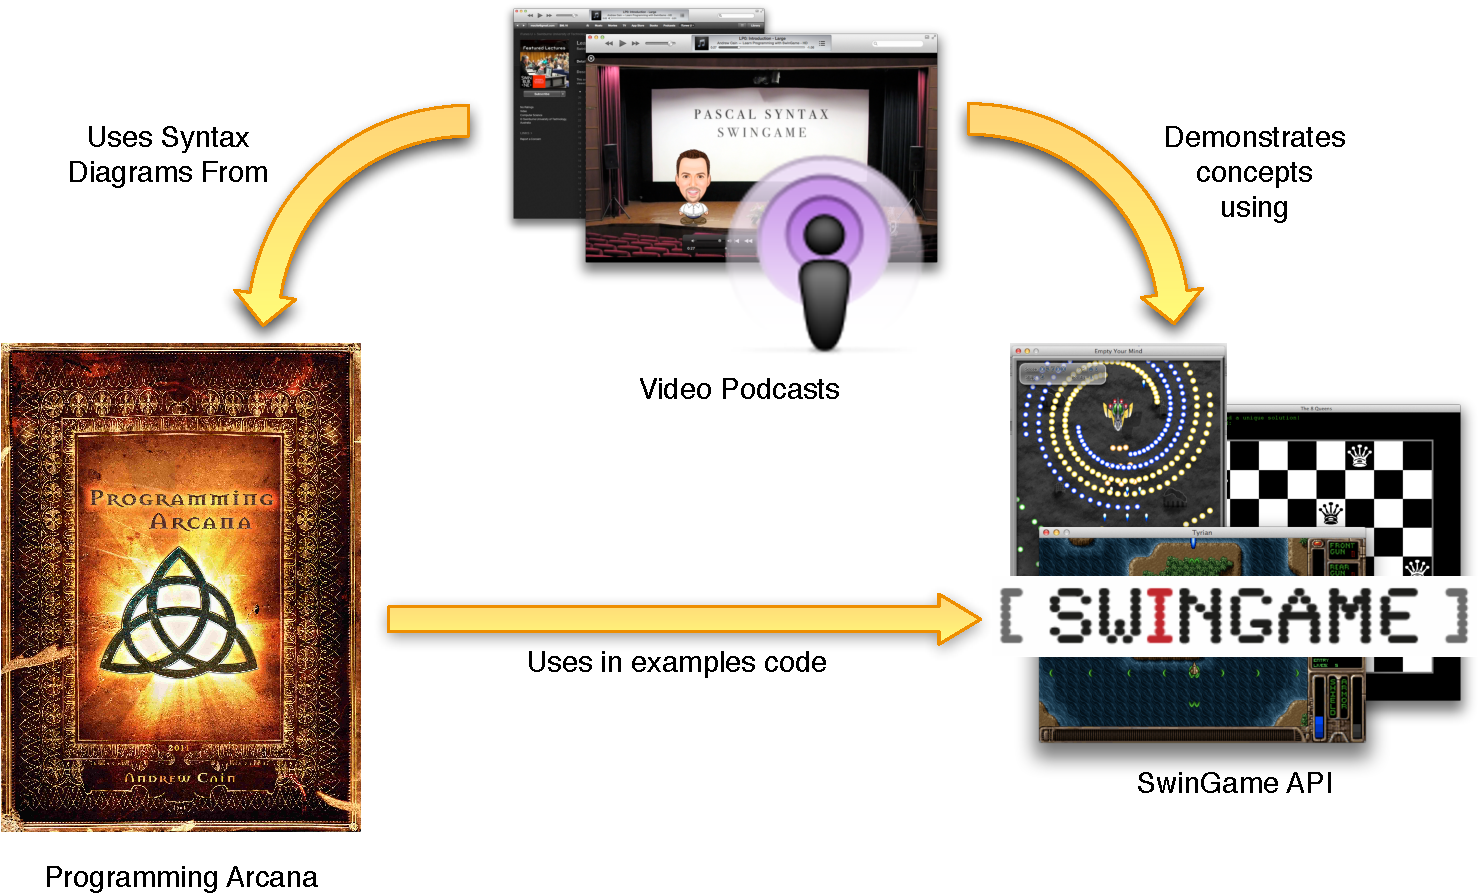
\includegraphics[width=0.8\textwidth]{SupportWhatWeTeach}
  \caption{SwinGame supported unit delivery, the Programming Arcana, and the video podcasts.}
  \label{fig:what_we_teach}
\end{figure}

% subsection supporting_what_we_teach (end)

\subsubsection{Evaluation and Support of Principles} % (fold)
\label{ssub:evaluation_and_support_of_principles}

Staff and student reflections indicate that SwinGame has been a successful part of the teaching strategy for the introductory and object oriented programming units. In the introductory programming unit SwinGame enabled staff to use interactive lecture demonstrations, and provided students with a library they could use to create small games for their custom projects. It supported the shift between programming languages, and between programming paradigms as student transition from the introductory programming unit to object oriented programming.

SwinGame has met most of the requirements listed in \sref{sub:swingame_requirements}, the following list outlines current strengths and weaknesses.
\begin{itemize}[noitemsep,nolistsep]
  \item Strengths:
  \begin{itemize}
    \item Provides required procedural, and object oriented, access to functionality to enable the creation of 2D games.
    \item Works cross platform, and across multiple languages.
    \item Device support includes desktop computers, and iOS devices (with touch and accelerometer support).
    \item Does provide support for drawing (shapes and images), audio, sprites, resource management, camera management, input, timers, networking, and physics.
    \item Does \textbf{not} take control away from the programmer -- less productive for better understanding.
  \end{itemize}
  \item Weaknesses (wish list):
  \begin{itemize}
    \item Documentation is very weak, developed by students early in their degree programmes.
    \item SwinGame is not highly optimised, being developed primarily by students.
    \item Needs support for a wider range of mobile devices, and support for additional input mechanisms.
    \item Does not support:
    \begin{itemize}[noitemsep,nolistsep]
      \item Image rotation and scaling, an often requested feature.
      \item Particle effects.
      \item Special effects, such as blur, fog, etcetera.
    \end{itemize}
    \item Lacks developer support beyond immediate teaching staff.
  \end{itemize}
\end{itemize}

SwinGame directly supported the programming units outlined in \cref{cha:example_impl}. Many of the lectures and weekly tasks in the introductory programming unit made use of the game library. Similarly, many of the early tasks in the object oriented programming unit used SwinGame as a means of learning the new language, and paradigm, without also needing to learn a new library. 

In terms of the principles stated in \cref{cha:guiding_principles}, and the model outlined in \cref{cha:approach}, SwinGame provided the following support:
\begin{itemize}[noitemsep,nolistsep]
  \item SwinGame helped realise the principles through:
  \begin{itemize}
    \item Interactive lecture demonstrations aimed to help guide students in the construction of their knowledge. (\Pref{itm:construct})
    \item Requiring explicit programmer control helped align SwinGame programming tasks with the programming concepts, and in turn the unit's intended learning outcomes. (\Pref{itm:align} and \Pref{itm:concepts})
    \item The consistent framework helped students overcome language differences, to better focus on programming concepts. (\Pref{itm:focus})
    \item Student involvement in the development of SwinGame provided a means of communicating high staff expectations. (\Pref{itm:expectations})
    \item SwinGame documentation, and simple interface, helped support student exploration of the library. (\Pref{itm:support})
    \item SwinGame helped staff engage with students, enabling them to guide lecture content. (\Pref{itm:theory_y})
    \item SwinGame provides procedural and object oriented programming abstractions, enabling it to be use in both procedural and object oriented programming languages. (\Pref{itm:paradigm} and \Pref{itm:authentic})
  \end{itemize}
  \item SwinGame helped implement the model in the example units by:
  \begin{itemize}
    \item Providing a valuable resource used in the teaching and learning activities of both programming units.
    \item Enabling students to develop a range of games for their custom projects.
    \item Providing a consistent library to help simplify the transitioning between languages.
    \item Supporting visual programming, making it easier for students to see when their programs were not working successfully.
  \end{itemize}
\end{itemize}

% add principles here

% subsubsection evaluation_and_support_of_principles (end)

\subsection{Summary} % (fold)
\label{sub:swingame_summary}

SwinGame provided a valuable resource in supporting students learning in the introductory programming units. The consistent library supported students transition between languages, interactive lecture demonstrations, and provided a wealth of features students could exploit in their custom programs. The strengths of SwinGame help maintain the focus on programming concepts. SwinGame remains an actively used library, and development continues to help address some of its current weaknesses.

% subsection summary (end)


% subsection use_of_swingame (end)


% section swingame_a_game_library_to_support_procedures_first (end)

\clearpage
\section{Programming Text to Support Concept-Based Approach} % (fold)
\label{sec:arcana}

Concepts are central to \emph{what} we aim to teach. \pref{itm:concepts} indicates that we should focus on concepts over language syntax. In addressing this principle the programming units from \cref{cha:example_impl} had little, if any, coverage of syntax in lectures, leaving these details instead to teaching and learning resources for students to use. These resources provide the syntax details students need to turn these concepts into working code.

One of the central ideas of ``Beyond Bullet Points'' is to fully document a presentation using the notes attached to a presentation's slides \cite{Atkinson:2007}. In effect, details are moved from a slide itself to the slides' notes area, which can then be printed as an informative handout. While documenting slides in this manner can provide students with the required details, it does mix the purpose of the presentation's slides as a means of guiding student thoughts and providing detailed information.

From our experience using the ``Beyond Bullet Points'' approach, this has a number of drawbacks in relation to the principles from \cref{cha:guiding_principles}. The dual purpose of the presentation works against maintaining a clear focus (\Pref{itm:focus}) as details may be better presented in a different order to the presentation slides, and visa versa. Similarly, the need for detailed notes for each slide works against \pref{itm:agile}, being agile and willing to change. The creation of the detailed notes results in significant effort being expended on the creation of each week's presentation, and thereby adds resistance to change if the presentation is found to be ineffective. 

Instead of documenting these notes in the presentations themselves, they were written up in a separate resource which became the ``\emph{Programming Arcana}'' \cite{Cain:2013arcana}. The title, cover image (see \fref{fig:front_cover_final}), and layout were designed around a magic theme in the aim of engaging students, they are becoming wizards of the modern era capable to making the computer do amazing things.

\begin{figure}[htbp]
  \centering
  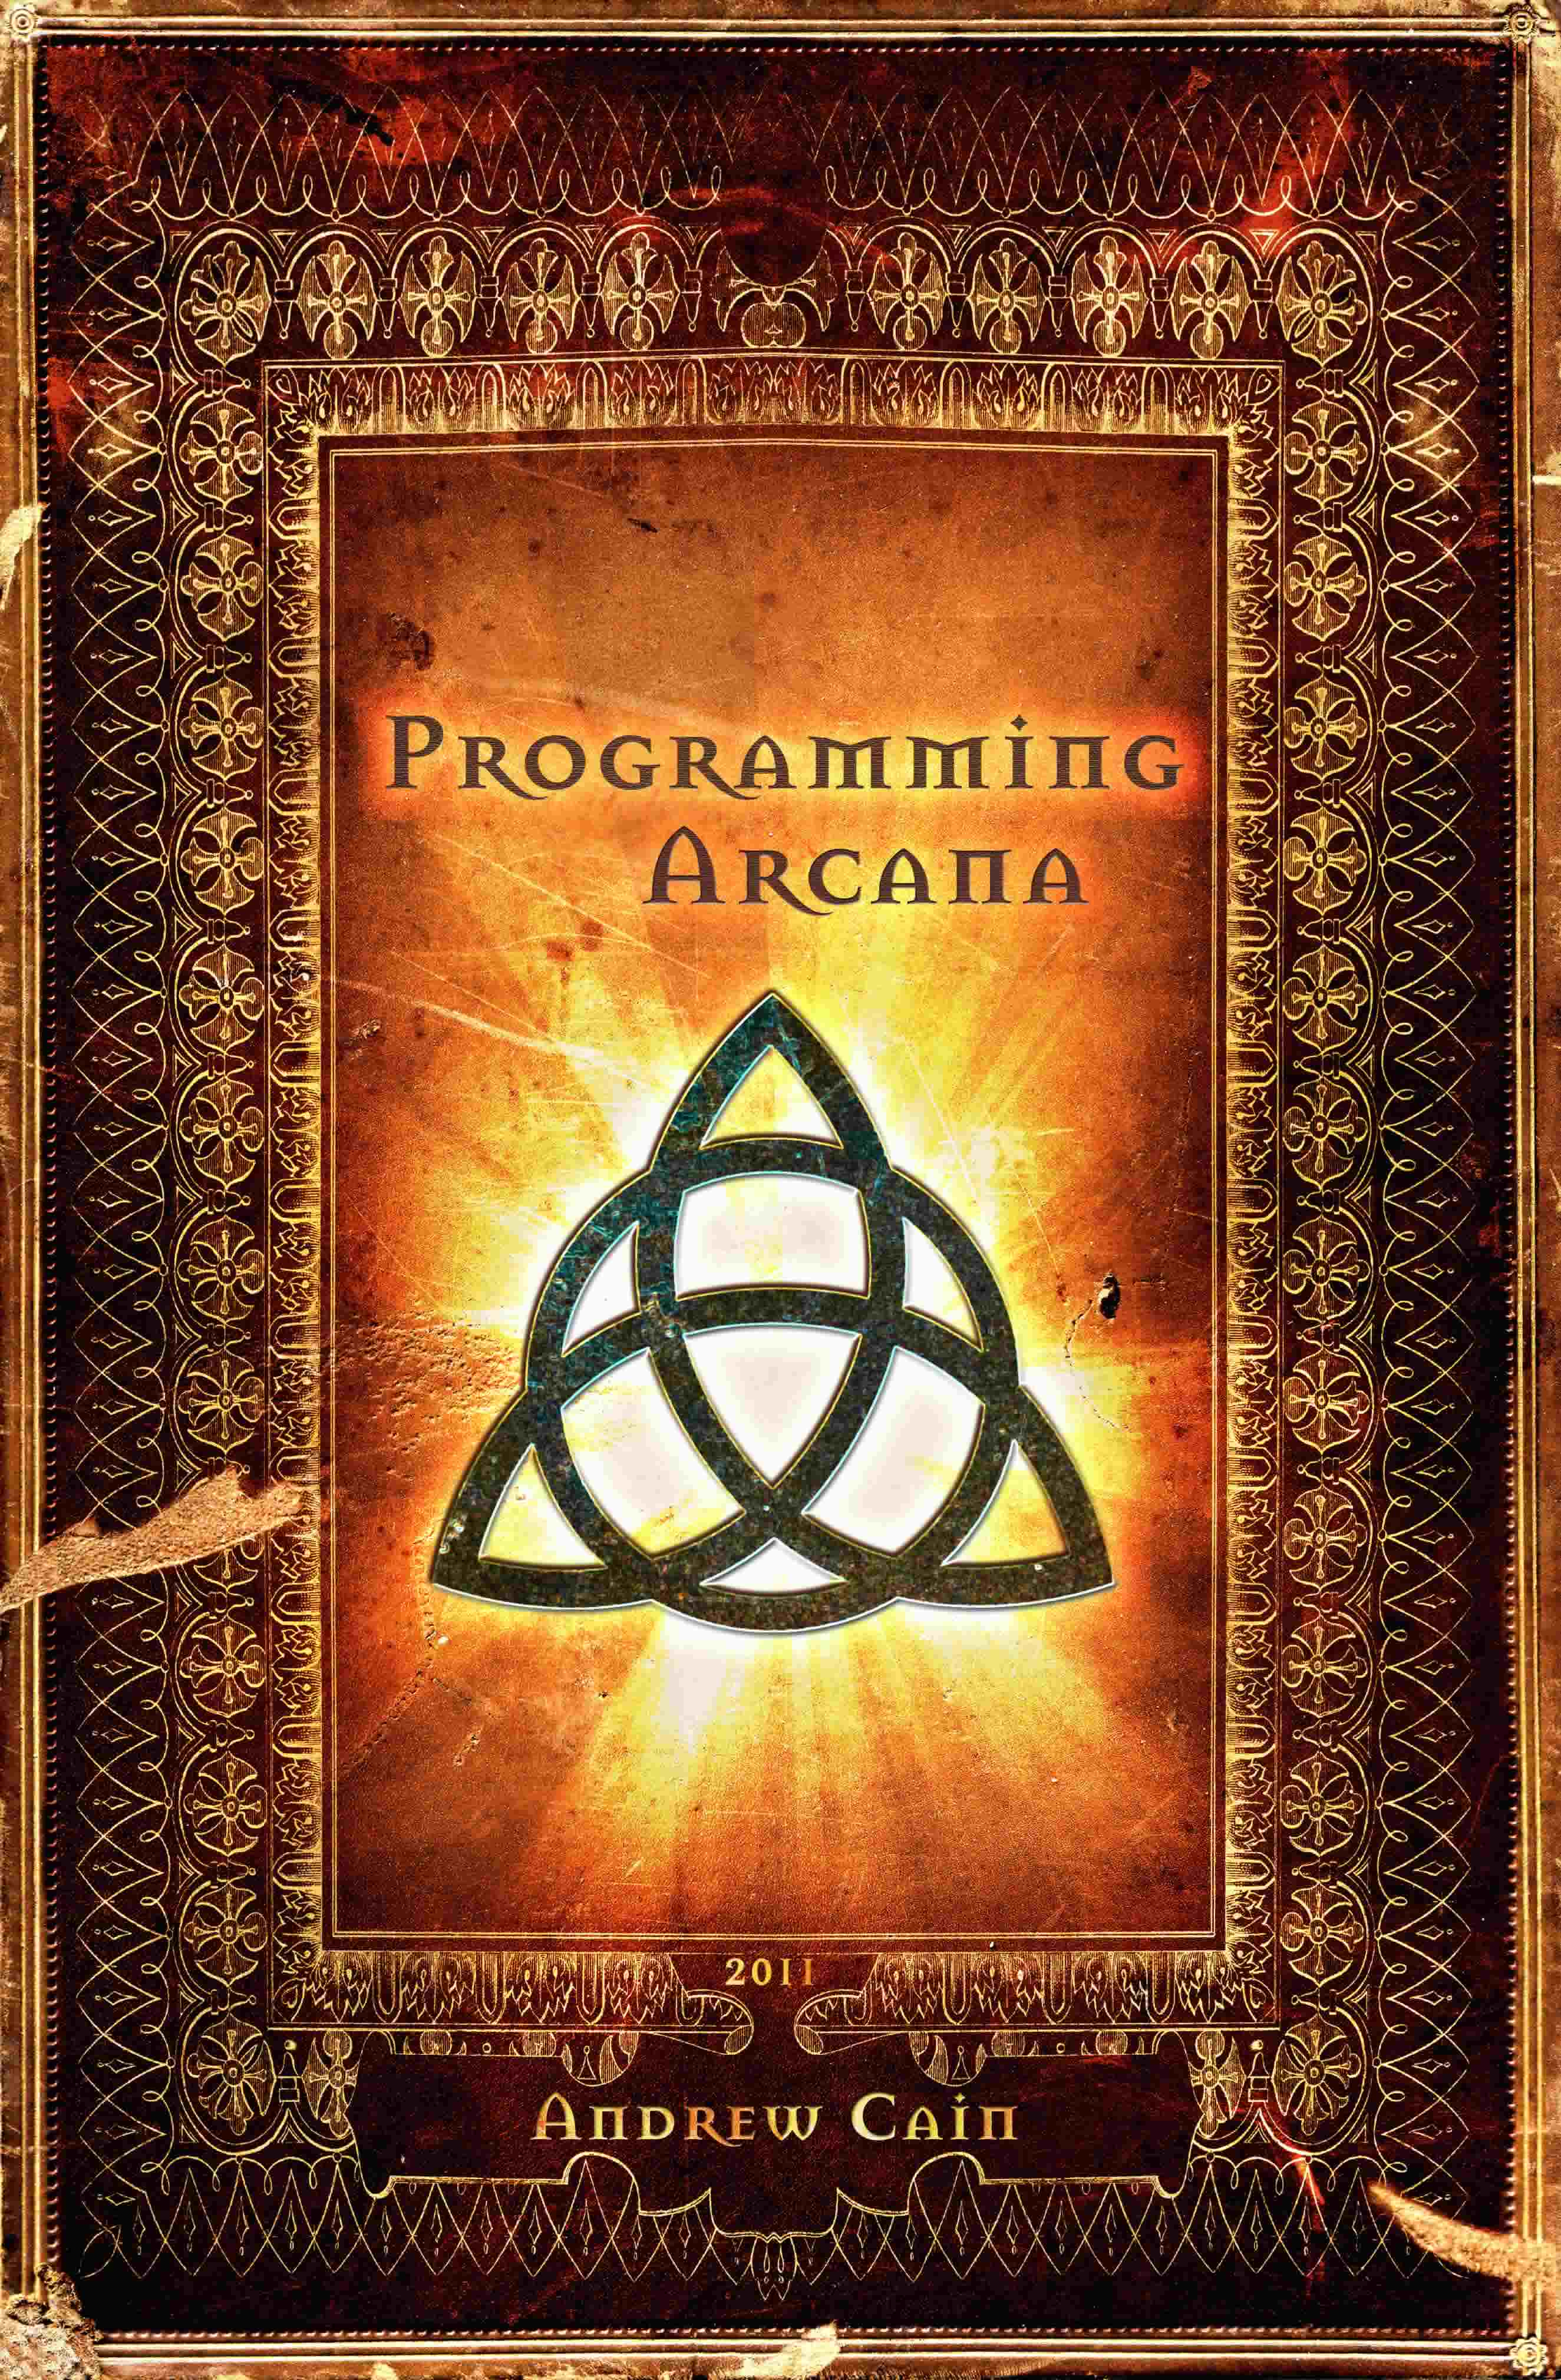
\includegraphics[width=0.4\textwidth]{front_cover_final}
  \caption{Front cover of the Programming Arcana, which used a magic theme to engage students as they worked towards becoming wizards with the computer.}
  \label{fig:front_cover_final}
\end{figure}

Documenting language details in a separate text from the presentations also helped to address another issue raised as a result of choosing Pascal as one of the programming languages. Pascal is not currently a popular language with institutions or text book writers, and while the Free Pascal Language Reference Guide \cite{FPC:2013lang} provides details of the language it is not designed for beginners. By providing our own text it was possible to maintain the concept-based ideas throughout all teaching and learning resources and activities, while also providing details on the Pascal and C languages, along with suitable programming examples.

This section outlines the requirements that the Programming Arcana aimed to met in \sref{sub:arcana_requirements}. \sref{sub:arcana_solution} describes the structure of the Programming Arcana, and the way in which it met its requirements. A short evaluation of the use of the Programming Arcana follows in \sref{sub:use_and_evaluation_of_the_programming_arcana}. This section then concludes with a brief summary in \sref{sub:arcana_summary}.

\subsection{Requirements} % (fold)
\label{sub:arcana_requirements}

The requirements for the Programming Arcana were to:
\begin{itemize}[noitemsep,nolistsep]
  \item Focus on programming concepts, presenting them in a language neutral manner.
  \item Order concepts to align with the introductory programming unit.
  \item Demonstrate application of the concepts to create a sample program, illustrating the thought process experts use.
  \item Provide syntax details to map concepts to code for the Pascal and C programming languages.
  \item Explain how the concepts operate on a notional machine.
  \item Provide sample code demonstrating applications of concepts, large and small.
  \item Be concise, focusing only aspects necessary to understand core ideas -- rather than presenting details on a range of possible options.
  \item Communicate ideas using a range of media.
\end{itemize}

% subsection requirements (end)

\subsection{Arcana Solution} % (fold)
\label{sub:arcana_solution}

\subsubsection{Chapter Sequence} % (fold)
\label{ssub:chapter_sequence}

Chapters in the Programming Arcana align with the concept topics from the introductory programming unit. This means that the text embodies the concept-based approach (\Pref{itm:concepts}) with each chapter providing a coherent set of concepts that build upon concepts presented earlier in the text. The following list outlines the main focus for each chapter. Additional details are provided in \aref{cha:chapters_from_the_programming_arcana} which lists the programming concepts that are presented in each of these chapters.

\begin{enumerate}[noitemsep,nolistsep]
  \item \textbf{Building Programs}: Introduces students to the tools they require, and shows them a basic, ``Hello World'', program they can compile to check that their tools are working.
  \item \textbf{Program Creation}: describes how code can be written to create a \emph{Program}.
  \item \textbf{Procedure Declaration}: Introduces the idea that you can create your own procedures to encapsulate the steps of a task. 
  \item \textbf{Storing and Using Data}: Makes programs more dynamic using variables and constants to store data, and functions to calculate values.
  \item \textbf{Control Flow}: Introduces structured programming principles, along with selection and repetition.
  \item \textbf{Managing Multiple Values}: Presents the use of arrays to make it easier to work with a large amount of data.
  \item \textbf{Custom Data Types}: Describes how developers can create types to help them organise the data in their programs, much as functions and procedures helped to organise functionality.
  \item \textbf{Dynamic Memory Allocation}: Extends programs beyond the confines of the stack, allowing the allocation of data on the heap.
  \item \textbf{Input and Output}: Describes how to save and load data from file.
\end{enumerate}

In proposing \pref{itm:concepts}, with its focus on programming concepts, \cref{cha:guiding_principles} outlined the requirement ``Introduce programming concepts incrementally.'' The Programming Arcana provides an example of how the details of a programming language can be presented in such a way as to ensure most topics are presented with each topic building upon the previously presented topics. 

\clearpage
There were two cases where concepts could not be suitably explained within the overall context presented in a chapter. There were:
\begin{enumerate}[noitemsep,nolistsep]
  \item In Chapter 1 the code for a working program was given to enable students to compile something before they understood what it represented. However, the main focus of the chapter was the tools being presented and not the specific details of the program's code, and so this does not directly contradict the underlying principle. 
  \item Chapters 2 and 3 makes use of values passed to procedures before topics related to \emph{how} data can be stored in a program. The idea that data can be passed to a procedure is covered, but not how that data was received, as the concept of a variable was not introduced until Chapter 4.
\end{enumerate}

Other than these two cases, all other chapters were able to explain all concepts in terms of the presented, or previously presented, concepts.

When comparing the suitability of the C and Pascal languages for supporting the concept-based approach it was noted that, in general, mapping the concepts to syntax was simpler for the Pascal programming language, with the C\footnote{The C code was compiled with a C++ compiler to add support for function and procedure overloading, and pass-by-reference.} language providing a number of challenges. C's standard input and output functions, \texttt{printf} and \texttt{scanf}, provided a range of challenges associated with the use of format strings and pointers. The format string provides an additional syntax to learn, and results in a range of runtime errors where the types indicated in the format string do not match the types of the associated variables or expressions. The need to pass explicit pointers to scanf also required a brief description of pointers in early material. Other challenges related to the need to understand arrays before working with strings. Early topics avoided strings, or used only string literals. In this way one example can be mapped to both C and Pascal languages. 

In relation to the use of the text in supporting the introductory programming unit, many of the issues with C were avoided due to the use of Pascal in the first part of the unit. This enabled teaching and learning activities to take advantage of Pascal's more convenient support for strings and terminal input and output. For example, consider a program that asked the user to enter their name and then echoes back a welcome message. In C this requires an understanding of variables, format string syntax, arrays, pointers, and how arrays are automatically passed by references. In Pascal the same program only requires an understanding of variables and pass-by-reference, as the language abstracts away many underlying details of how strings work.

% subsubsection chapter_sequence (end)
\clearpage
\subsubsection{Chapter Layout} % (fold)
\label{ssub:chapter_layout}

Each chapter of the Programming Arcana has a similar sequence to its sections, with the intention of reducing cognitive overhead and promoting a consistent approach to studying each of the topic. In keeping with \pref{itm:concepts}, the concepts were presented as the focus of each chapter.

\begin{enumerate}[noitemsep,nolistsep]
  \item \textbf{Concepts}: Each chapter starts with a list of related concepts, each of which is described at a relevant level of detail for that chapter.
  \item \textbf{Applying the Concepts}: An example of how to apply the chapter's concepts is then discussed, using pseudocode and flowcharts to illustrate how the concepts can be applied.
  \item \textbf{Syntax in C and Pascal}: Details related to the syntax needed to realise these concepts in code are first presented for the C programming language, and then for the Pascal language.
  \item \textbf{Understanding the Concepts}: Traces the execution of the pseudocode on a conceptual machine, with the aim of showing students how the concepts are realised at run time. 
  \item \textbf{Examples}: A number of examples are given to further demonstrate the application of the chapter's concepts, each is presented in pseudocode and then in C and Pascal code.
  \item \textbf{Exercises}: Provides a sequence of exercises students can use to develop their understanding of the topic.
\end{enumerate}

Details of the sections related to presenting the concepts follow. This outlines how the Programming Arcana implemented the concept-based approach, and reinforce the focus on concepts over syntax throughout the material presented. 

\clearpage
\paragraph{Concepts} % (fold)
\label{par:concepts}

Each chapter starts with a section that provides details of the concepts being presented. This starts with a brief overview describing how all of the concepts are related, with following subsections presenting details for each concept. Concepts are presented using a textual description, visual concept map, and a series of notes with important details related to the topic. At the end of the concept section an overall concept map is included to visually summarise the relationships between the concepts covered. 

\fref{fig:arcana_concepts} shows an example of the concept of branching from Chapter 5 of the Programming Arcana. The diagrams were deliberately drawn using irregular, rough looking, shapes to indicate these were a conceptualisation, rather than an exact representation of the associated concepts.

One of the design goals was to fit each concept on a single page. This goal aimed to help support a student's active construction of knowledge, \pref{itm:construct}. Aiming to keep each topic to a single page ensured a focus (\pref{itm:focus}) on the most important details, and where topics expanded over multiple pages the details were examined to ensure they did not included any unnecessary details.

\begin{figure}[h]
  \centering
  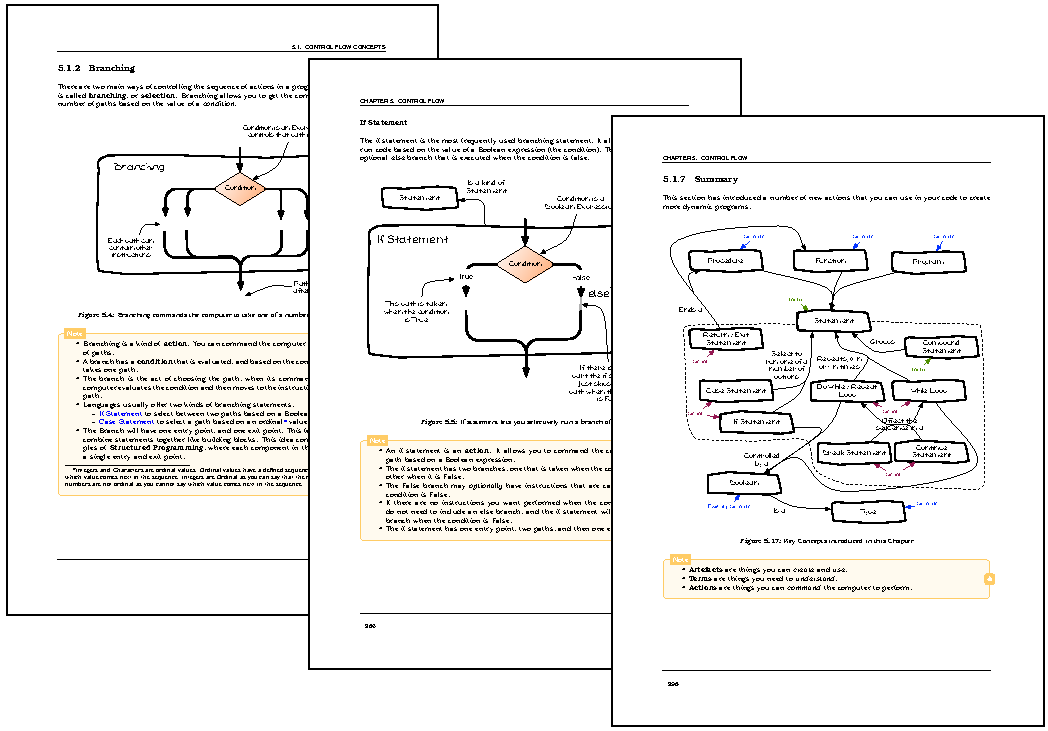
\includegraphics[width=0.95\textwidth]{ArcanaConcepts}
  \caption{Example concept pages from Chapter 5 of the Programming Arcana, showing the use of visual concept maps to help explain concepts. }
  \label{fig:arcana_concepts}
\end{figure}

% paragraph concepts (end)
\clearpage
\paragraph{Applying the Concepts} % (fold)
\label{par:applying_the_concepts_}

After the concepts are presented, the next section outlines how these concepts work together to create an example program. This helps demonstrate the thought process of an expert programmer in applying these concepts to a program design, with the aim of helping students construct similar thought patterns (\Pref{itm:construct}). This section starts with a specification of a program to be created. This is then followed by a discussion of how a program can be designed using the concepts covered to that point in the text. The description of the design includes pseudocode, flow charts, sequence diagrams and structure charts, and the section concludes with a complete design for the specified program. \fref{fig:arcana_applying} shows an example of designing a ``Guess that Number'' game that demonstrates the application of control flow concepts.

\begin{figure}[h]
  \centering
  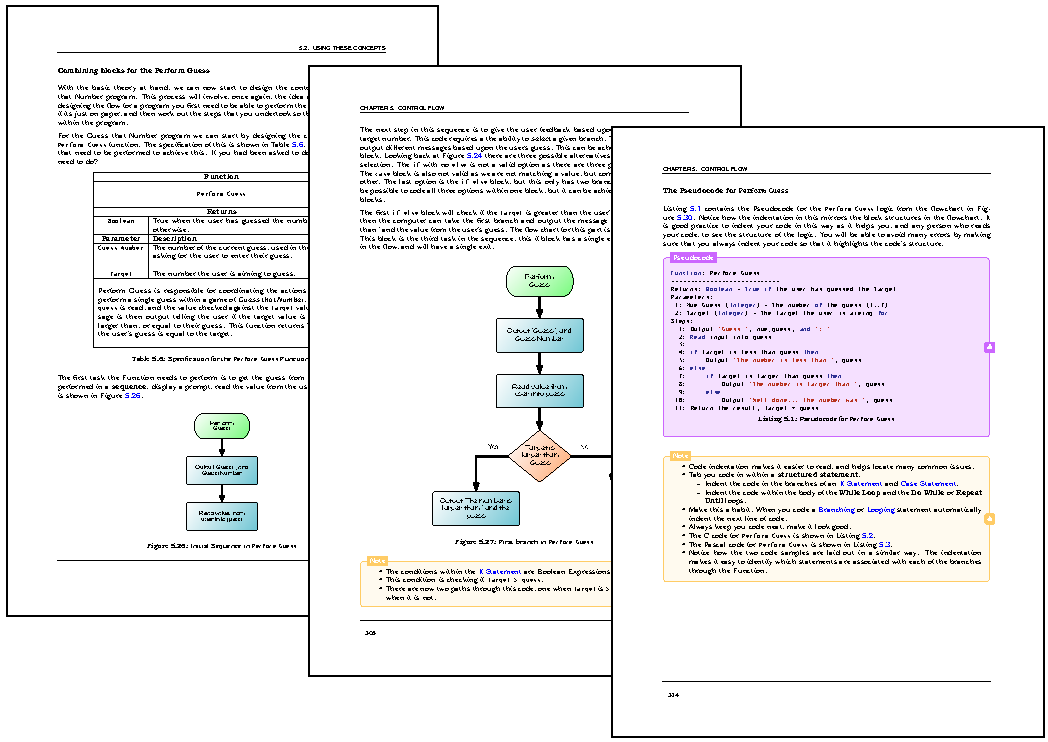
\includegraphics[width=0.95\textwidth]{ArcanaApplying}
  \caption{Example pages related to applying the concepts from the Programming Arcana}
  \label{fig:arcana_applying}
\end{figure}

In each chapter explanatory text accompanies the design, and highlights how the concepts covered contribute to the end result. This discussion also presents a way of approaching problems using the concepts to introduce students to the ideas they can use in approaching the design of their own programs.

% paragraph applying_the_concepts_ (end)
\clearpage
\paragraph{Syntax} % (fold)
\label{par:syntax}

Having covered concepts, and how they can be used to design a program, the next two sections deal with realising these concepts using the C and Pascal programming languages. The syntax sections start with an implementation of the program designed in the section on applying the concepts, in this way students see design through to its implementation with the aim of helping them develop appropriate conceptual connections (\Pref{itm:construct}). This is followed by details of each part of the language syntax, providing this section with a clear focus (\Pref{itm:focus}). An example of pages from this section is shown in \fref{fig:arcana_syntax}.

\begin{figure}[h]
  \centering
  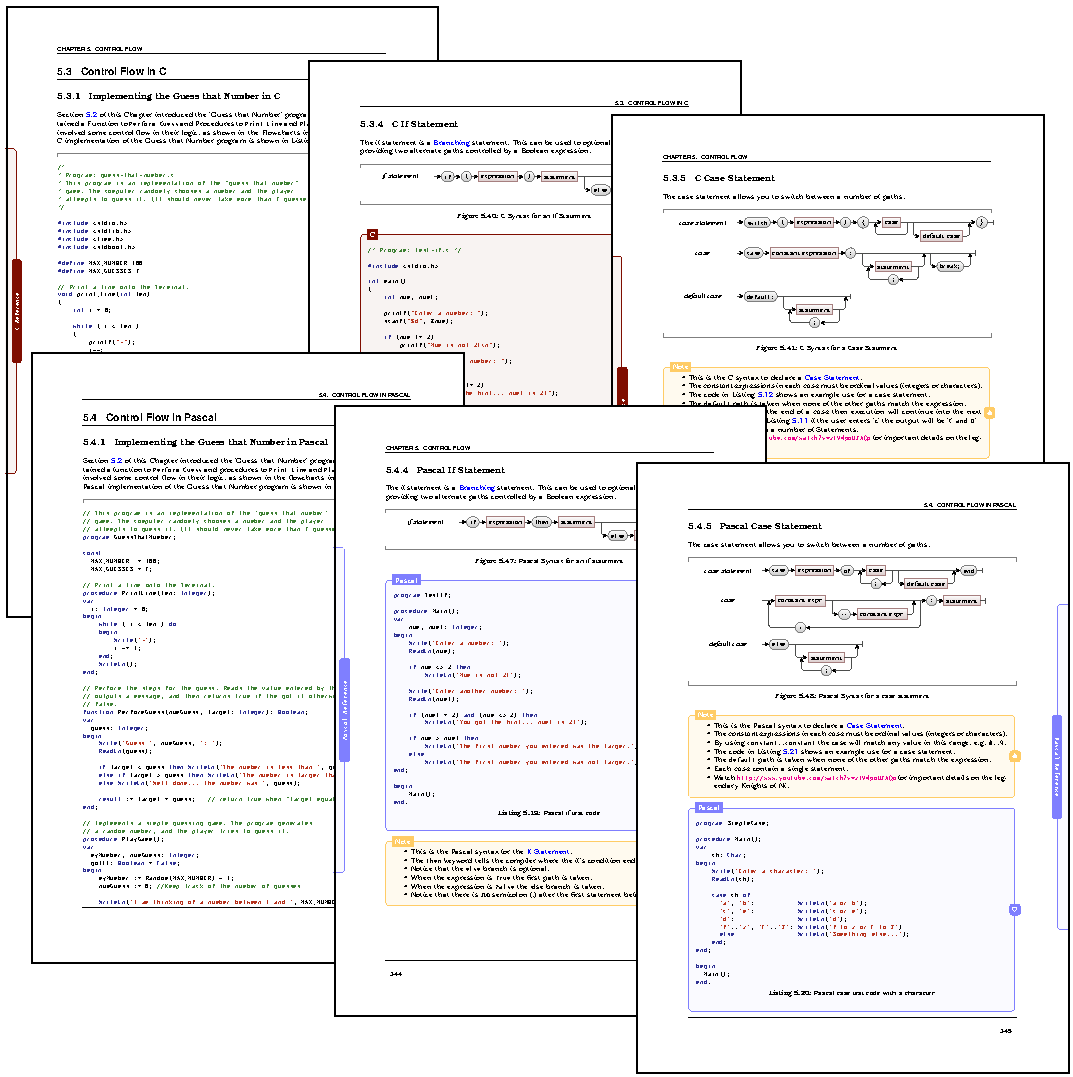
\includegraphics[width=0.95\textwidth]{ArcanaSyntax}
  \caption{Example pages from the Programming Arcana showing C and Pascal syntax and examples}
  \label{fig:arcana_syntax}
\end{figure}

Maintaining a clear focus on the most important aspects continues in the presentation of the syntax (\Pref{itm:focus}). The design aimed for each aspect of the syntax to be presented in a single page. The grammar, and examples, presented focus on best representing the concepts, which in many cases means only presenting a small subset of what is possible with the programming language. 

% paragraph syntax (end)

\paragraph{Understanding the Concepts} % (fold)
\label{par:understanding_the_concepts_}

In order to think and act as experts, the goal of constructivist education, it is important for students to understand how the instructions affect the machine they are programming (\Pref{itm:construct}). This imperative was highlighted by \citet{BenAri:1998,BenAri:2001} in their analysis of constructivism in computer science education, in which they indicated the critical importance of ensuring students develop an effective model of computation. For the introductory programming unit, the intended learning outcomes indicated that students need to be able to \emph{explain} their programs, this aimed to encourage students to develop, and communicate, their model of computing, and required resources they could draw upon to highlight these lower level operations (\Pref{itm:align}).

The notional machine represents an ideal computer in which the programming constructs being taught are realised \cite{DuBoulay:1986}. To help students realise the goal of \emph{understanding} how to program this machine, the next section of each chapter in the Programming Arcana provided a series of illustrations. These illustrations aim to communicate the state and behaviour of the notional machine as it executes the example program developed in earlier sections. \fref{fig:notional_machine} shows an example of the notional machine from the Programming Arcana, the machine contains a persistent storage device, central processing unit (CPU), terminal for input and output, and memory that is divided into sections for global values, stack, instructions, and heap -- in later chapters. 

\begin{figure}[p]
  \centering
  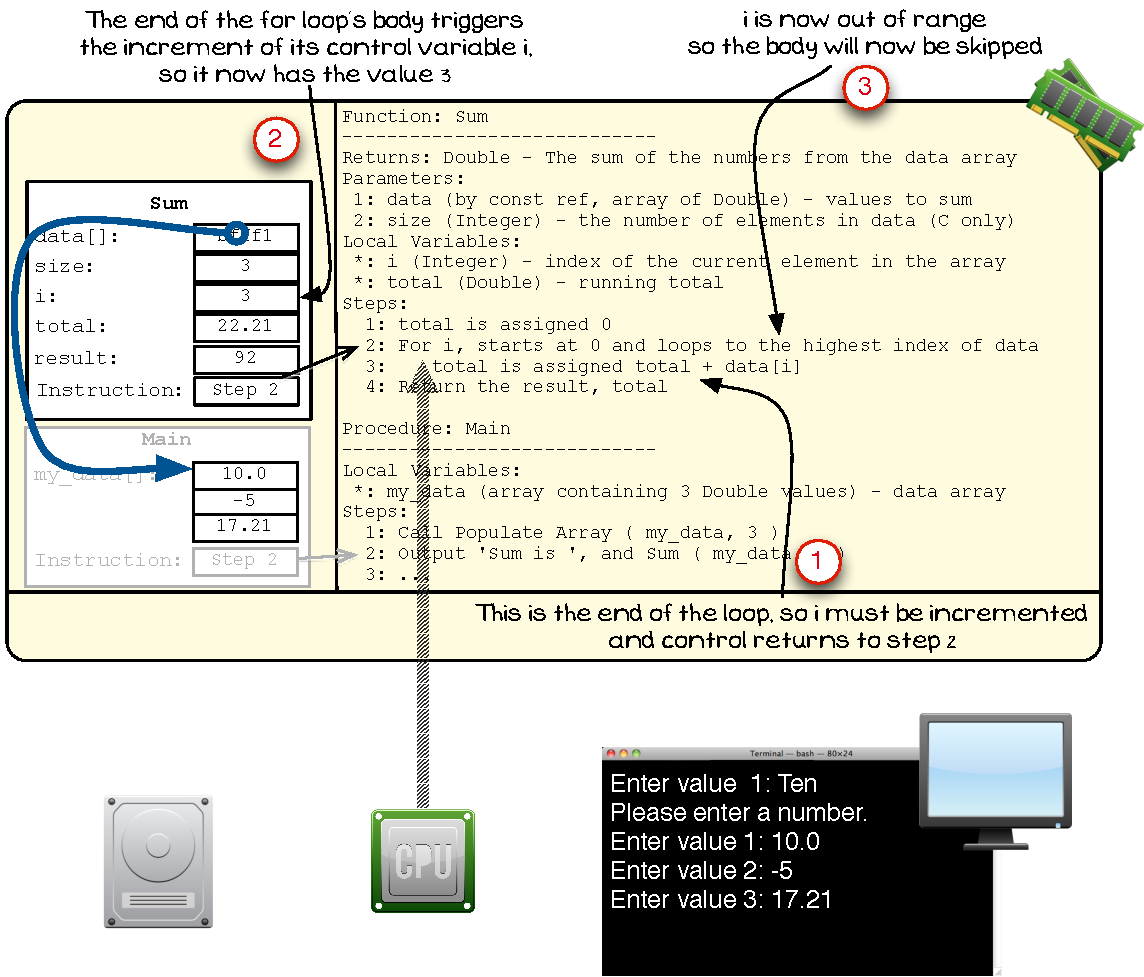
\includegraphics[width=0.8\textwidth]{NotionalMachine}
  \caption{Example of the visualisation of the notional machine used in the Programming Arcana}
  \label{fig:notional_machine}
\end{figure}


\fref{fig:arcana_understanding} shows some examples from the chapter on control flow. The illustration of the notional machine focuses on memory, and the instruction the computer is executing. Instructions from the pseudocode are executed, one by one, with each instruction being explained on a single page. The state of the machine is discussed after each instruction, with each page including a short description of what is occurring, a visualisation of the notional machine, related notes on the steps taken by the machine, and any language specific notes. Annotations were added to the visualisation of the notional machine to help link the comments to changes in the machine's state.

\begin{figure}[p]
  \centering
  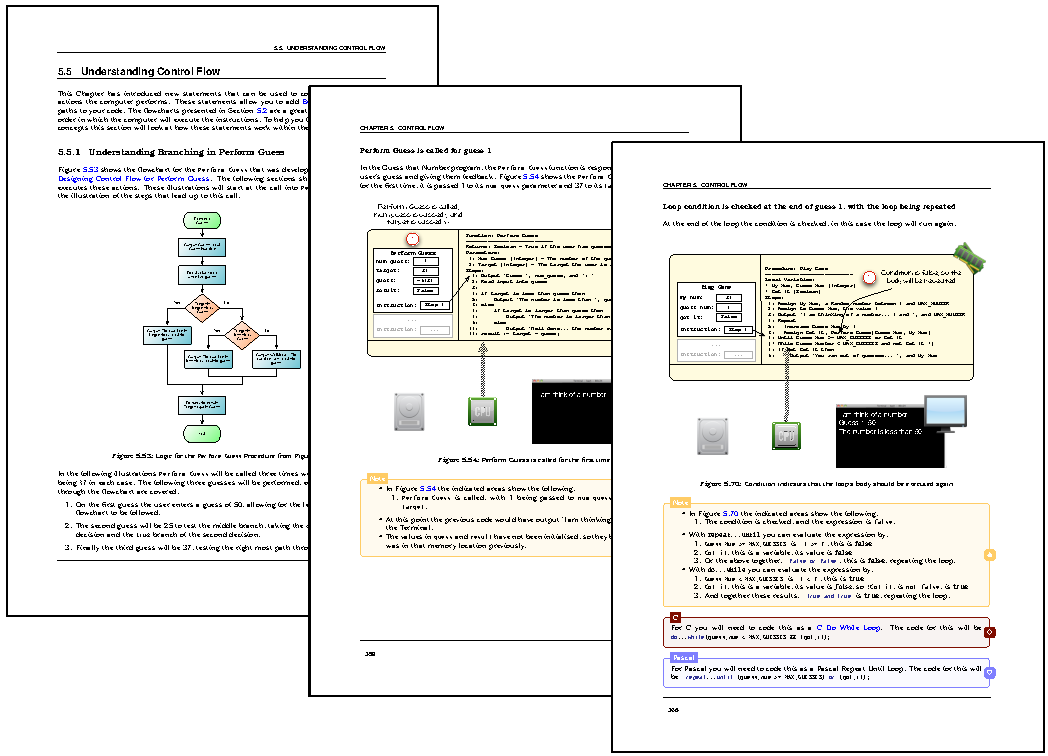
\includegraphics[width=0.95\textwidth]{ArcanaUnderstand}
  \caption{Examples pages from the Programming Arcana illustrating how the concepts worked to instruct the notional machine}
  \label{fig:arcana_understanding}
\end{figure}

% paragraph understanding_the_concepts_ (end)

% subsubsection chapter_layout (end)


\clearpage
\subsection{Use and Evaluation of the Programming Arcana} % (fold)
\label{sub:use_and_evaluation_of_the_programming_arcana}

The Programming Arcana was able to meet all of its core requirements, though the use of multiple media formats could be enhanced if the book transitioned to an e-book format. Reflections from teaching staff indicate that it has provided a valuable tool in teaching the introductory programming unit. Staff have received a number of messages from students indicating how valuable they found the resource, a sentiment often reflected in reflections from student portfolios. The following list outlines how the Programming Arcana helped with the delivery of the example units, supported the model described in \cref{cha:approach}, and reflected the principles stated in \cref{cha:guiding_principles}.

\begin{itemize}[noitemsep,nolistsep]
  \item The Programming Arcana embodies the following principles:
  \begin{itemize}[noitemsep,nolistsep]
    \item Explanations aim to guide students to deeper understanding of the concepts associated with the introductory programming unit. (\Pref{itm:construct}, \Pref{itm:align}, and \Pref{itm:concepts})
    \item Each section focuses on important aspects, avoiding unnecessary details. (\Pref{itm:focus})
    \item Examples and explanations of concepts, syntax, and execution help support student learning. (\Pref{itm:support})
    \item Resources from the Programming Arcana provided material used in lecture notes. (\Pref{itm:agile})
    \item The Programming Arcana focuses on communicating procedural programming concepts, in an appropriate manner for the two programming languages. (\Pref{itm:paradigm} and \Pref{itm:authentic})
    \item Chapters are organised so that later chapters built upon concepts presented in earlier chapters. (\Pref{itm:concepts})
  \end{itemize}
  \item The Programming Arcana supported the use of the model in delivering the introductory programming unit by:
  \begin{itemize}[noitemsep,nolistsep]
    \item Providing details that were removed from lectures, to enable these to be more interactive.
    \item Aligning content presented in the text, with the material from lectures and core tasks, thereby providing a consistent experience for students.
    \item Supporting the focus on concepts, providing students with additional explanations and examples.
    \item Providing resources to aid students with the core tasks.
  \end{itemize}
\end{itemize}

% subsection use_and_evaluation_of_the_programming_arcana (end)

\clearpage
\subsection{Summary} % (fold)
\label{sub:arcana_summary}

The Programming Arcana textbook demonstrates how the concept-based approach of the model can be embedded down to the syntax level. The text provides students with the details related to programming concepts, how they apply to program design, the associated syntax, and details on how they work within a notional machine. A range of learning styles are supported through the presentation of the syntax and concepts using both images and text. Overall, the Programming Arcana supported the concept-based approach to teaching introductory programming by providing students with details on the concepts, their application, syntax and operations. 

% subsubsection summary (end)


% subsection programming_arcana (end)
\section{Video Podcasts to Support the Programming Text} % (fold)
\label{sec:vodcasts}

While it was able to meet most of its requirements, the one area where the Programming Arcana was limited was its use of static text and images, a limitation of its format. To provide students with an alternative medium, a number of video podcast series were created and made available to students via iTunesU. Three series were created in total, and each took a different approach to what should be presented. The first series, ``Object Oriented Programming'', covers object oriented programming principles and focused on communicating these concepts with little coverage of language syntax. ``Learning Programming with SwinGame'' was the second series created, and focuses on communicating Pascal syntax. The third series, ``Introductory Programming'', focuses on a combination of the two, presenting the concepts and the syntax together. Each of these series is discussed in the following subsections.

\subsection{Requirements} % (fold)
\label{sub:vodcast_requirements}

The following list outlines the requirements for the video podcasts. This is divided into general requirements for all podcasts, and specific requirements for the individual series.

\begin{itemize}[noitemsep,nolistsep]
  \item All video podcasts were required to:
  \begin{itemize}[noitemsep,nolistsep]
    \item Clearly present a number of concepts or syntax.
    \item Provide live coding demonstrations.
    \item Be small in size, enabling fast downloads, while ensuring code was still readable.
    \item Incorporate Swinburne's introduction and summary video material.
    \item Be accessible published to iTunesU with associated meta-data.
  \end{itemize}
  \item The Object Oriented Programming series was required to:
  \begin{itemize}[noitemsep,nolistsep]
    \item Provide all content traditionally delivered in lectures.
    \item Enable a classroom ``flip'', where lectures are used to discuss content and the video podcast takes the place of the traditional lecture.
  \end{itemize}
  \item The Learn Programming with SwinGame series was required to:
  \begin{itemize}[noitemsep,nolistsep]
    \item Demonstrate Pascal programming syntax.
    \item Each video should focus on a single piece of syntax, and demonstrate its use in general and in relation to programming small games.
  \end{itemize}
  \item The Introductory Programming series was required to:
  \begin{itemize}[noitemsep,nolistsep]
    \item Provide a summary of lecture content of lecture content.
    \item Demonstrate C programming syntax.
  \end{itemize}
\end{itemize}

% subsection requirements (end)

\subsection{Video Podcasts Solution} % (fold)
\label{sub:video_podcasts_solution}

Each of the Video Podcast series was developed using a number of video editing tools. Video from coding demonstrations, images of presentation slides, voice over audio, and character animations were all combined together in the video editing software to create each video podcast. Typical processing involved first recording coding demonstrations, and exporting presentation slides, then recording voice over audio. There were then combined with a video editing tool, which involved adjusting slide and video speed to match audio.

\tref{tbl:vodcasts} provides an overview of the three podcast series. The Object Oriented Programming series was used by the object oriented programming unit, and provided traditional lecture style content. Learning Programming with SwinGame focused on presenting Pascal programming language syntax, as a more dynamic extension of the Programming Arcana. Whereas the Introductory Programming series provided both lecture style content, and coding demonstrations.

\begin{table}[htbp]
  \centering
  \caption{Video podcast series details}
  \label{tbl:vodcasts}
  \begin{tabular}{l|c|r}
  \textbf{Series Name} & \textbf{Episodes} & \textbf{Episode Length} \\
  \hline
  Object Oriented Programming & 19 & 6-36 minutes \\
  Learning Programming with SwinGame & 26 & 2-15 minutes \\
  Introductory Programming & 7 & 17-38 minutes \\
  \end{tabular}
\end{table}

\subsection{Use and Evaluation of Video Podcasts} % (fold)
\label{sub:use_and_evaluation_of_video_podcasts}

All three podcast series were used to support students learning in the example units discussed in \cref{cha:example_impl}. The podcasts provided students with an alternative medium for approaching the concepts and syntax that was included in the Programming Arcana, with the expectation that students would be able to use both resources to support the construction of their knowledge.

The following list relates the video podcasts to the principles stated in \cref{cha:guiding_principles}.
\begin{itemize}[noitemsep,nolistsep]
  \item Video podcasts provided an additional source of material students could use to help construct their own knowledge. (\Pref{itm:construct})
  \item Content presented in the video podcasts aligned with the intended learning outcomes of the example programming units. (\Pref{itm:align})
  \item The video podcasts provided another set of resources to help support student learning efforts. (\Pref{itm:support})
  \item In each case, episodes demonstrate appropriate use of programming languages. (\Pref{itm:authentic})
\end{itemize}

In addition to the above list, it was felt that the Learning Programming with SwinGame series had also demonstrated use of the following principles. These principles were not present in the other series which tended to focus on information provision, with a wider set of concepts. 
\begin{itemize}[noitemsep,nolistsep]
  \item Episodes focused on demonstrating a single statement, and provided a number of examples to illustrate its use. (\Pref{itm:focus})
  \item The small focus of these podcasts helped reduce time needed to produce the series. The specific nature of the series also allowed it to be re-used when activities and lecture sequences changed. (\Pref{itm:agile})
  \item Podcasts provided support for language syntax, allowing other activities to focus on underlying concepts. (\Pref{itm:concepts})
\end{itemize}

Interestingly, the Learning Programming with SwinGame series proved to be the most useful of the three series. Its clear focus on communicating programming syntax allowed it to be used more flexibly, as it did not depend on other teaching and learning activities. In contrast, the other two series inclusion of concepts meant that they had a greater dependence on how, and in which order, topics were covered in the unit. The use of a larger number of more specific episodes in the Learning Programming with SwinGame series, also made it easier to incorporate the videos in relevant lecture and laboratory notes.

Teaching staff indicated that future video podcasts would continue to use the format of the Learning Programming with SwinGame series. Specifically, the narrow focus and short duration. New series are currently planned to help demonstrate how to achieve certain effects in game programs developed using the SwinGame library. These podcasts would demonstrate how to combine a number of concepts in creating slightly larger programs.

% subsection use_and_evaluation_of_video_podcasts (end)

\subsection{Summary} % (fold)
\label{sub:vodcast_summary}

Video podcasts provided students with an alternative means for studying unit concepts and programming language syntax. It was found that specific, short duration, podcasts had a longer lifespan as they worked together with teaching and learning activities.


% subsection supporting_multiple_modes_of_learning (end)

% subsection video_podcasts_solution (end)




% subsection vodcasts (end)

% section itunesu_vodcasts_to_support_ (end)
\section{Chapter Summary} % (fold)
\label{sec:supporting_summary}

This chapter has discussed four resources used to support \emph{how} and \emph{what} was taught in the example units from \cref{cha:example_impl}. Doubtfire helped to support the use of formative feedback during the semester, with visual feedback being used in lieu of marks to help motivate students. SwinGame provided a game library to help students create rich and interactive programs. The Programming Arcana provided students with details on the concepts, their application, associated syntax, and operation on the notional machine. Which was also supported by the video podcasts, which provided students with an alternative means of study.

\cref{cha:evaluation} presents a further evaluation of these resources, the teaching and learning activities from \cref{cha:example_impl}, and model from \cref{cha:approach}.

% section summary (end)


% chapter supporting_the_curriculum (end)